\pdfoutput=1
\newpage
\section*{Appendix Table of Contents}

\begin{itemize}
    \item \ref{related_work} Related work \dotfill \pageref{related_work}
    \begin{itemize}
      \item \ref{related_work:single_llm} Single LLM Reasoning \dotfill \pageref{related_work:single_llm}
      \item \ref{related_work:multi_llm} Multiple LLM Reasoning \dotfill \pageref{related_work:multi_llm}
      \item \ref{related_work:hrl_reason} Hierarchical Reasoning \dotfill \pageref{related_work:hrl_reason}
      \item \ref{related_work:rl_in_llm} RL in LLM \dotfill \pageref{related_work:rl_in_llm}
    \end{itemize}
    \item \ref{sec:limitation_and_future_work} Limitation and Future Work \dotfill \pageref{sec:limitation_and_future_work}
    \item \ref{app:suppl_method} Supplementary Materials for Method in Section~\ref{sec:method} \dotfill \pageref{app:suppl_method}
    \begin{itemize}
        \item \ref{sec:appx.reinforce_ma.infer_scaling} Inference-time Scaling For \method \dotfill \pageref{sec:appx.reinforce_ma.infer_scaling}
        \item \ref{app:reward_design} Detailed reward design \dotfill \pageref{app:reward_design}
        \item \ref{app:pseudocode} Pseudocode of \method \dotfill \pageref{app:pseudocode}
        \item \ref{app:convergence_analysis} Brief convergence analysis \dotfill \pageref{app:convergence_analysis}
        \item \ref{sec:app_lfg} Learning to reason from the perspective of Leader Follower Game \dotfill \pageref{sec:app_lfg}
    \end{itemize}
    \item \ref{app:exp_setting} Training Details \dotfill \pageref{app:exp_setting}
    \begin{itemize}
        \item \ref{app:exp_setting.single_turn_rema} Single-turn ReMA \dotfill \pageref{app:exp_setting.single_turn_rema}
        \begin{itemize}
            \item \ref{app:exp_setting.single_turn_rema.sft_data} Supervised fine-tuning data collection \dotfill \pageref{app:exp_setting.single_turn_rema.sft_data}
            \item \ref{app:exp_setting.single_turn_rema.rewardbench970} Dataset Curation of RewardBench970 \dotfill \pageref{app:exp_setting.single_turn_rema.rewardbench970}
            \item \ref{app:exp_setting.single_turn_rema.math} Training on MATH \dotfill \pageref{app:exp_setting.single_turn_rema.math}
            \item \ref{app:exp_setting.single_turn_rema.reward_bench} Training on Reward Bench \dotfill \pageref{app:exp_setting.single_turn_rema.reward_bench}
        \end{itemize}
        \item \ref{app:exp_setting.multi_turn_rema} Multi-turn ReMA \dotfill \pageref{app:exp_setting.multi_turn_rema}
        \begin{itemize}
            \item \ref{app:exp_setting.multi_turn_rema.sft_data} SFT data collection of multi-turn MAMRP \dotfill \pageref{app:exp_setting.multi_turn_rema.sft_data}
            \item \ref{app:exp_setting.multi_turn_rema.math} Training on MATH \dotfill \pageref{app:exp_setting.multi_turn_rema.math}
        \end{itemize}
    \end{itemize}
    \item \ref{app:other_exp} Other Experiments \dotfill \pageref{app:other_exp}
    \begin{itemize}
        \item \ref{exp:reward_design} Reward functions shape cross-agent behaviors \dotfill \pageref{exp:reward_design}
        \item \ref{app:exp_setting.multi_turn_rema.detailed_training_curves} Detailed Training Curves on Different Datasets of Multi-turn \method \dotfill\pageref{app:exp_setting.multi_turn_rema.detailed_training_curves}
    \end{itemize}
    \item \ref{app:qualitative_results} Qualitative results \dotfill \pageref{app:qualitative_results}
    \begin{itemize}
        \item \ref{app:qualitative_results.high_level_better} High-level policy finds better plans \dotfill \pageref{app:qualitative_results.high_level_better}
        \item \ref{app:qualative_results.case_study} Case study for Experiments of Different Reward Functions in Appendix~\ref{exp:reward_design} \dotfill \pageref{app:qualative_results.case_study}
        \item \ref{app:qualative_results.case_study.json} Case study for Adaptive Meta-thinking in Single-Turn \method~in Section~\ref{sec:exp.high_rl} \dotfill \pageref{app:qualative_results.case_study.json}
    \end{itemize}
    \item \ref{app:prompts} Prompts \dotfill \pageref{app:prompts}
\end{itemize}

\pdfoutput=1

\section{Related work}
\label{related_work}

% Researchers have explored several classes of methods to enhance LLM reasoning. Single-agent approach falls into two categories: search-based \citep{brown2020language,graves2012sequence,snell2024scaling,wang2022self,lightman2023let} and post-training methods \citep{qin2024o1replicationjourneystrategic, ouyang2022training, hui2024qwen2, liu2024deepseek,wang2024openr, zhang2024llamaberrypairwiseoptimizationo1like, r1, xu2025towards}. Multi-agent approach includes aggregating static knowledge from off-the-shelf LLMs \citep{zhang2025if,chen2024s,du2023improving,liang2023encouraging,hong2023metagpt,zhang2024aflow} and improving reasoning ability via training \citep{ma2023red,kirchner2024prover}. Hierarchical reasoning approach further partitions reasoning into hierarchical processes \citep{saha2025learningplanreason,DBLP:journals/corr/abs-2410-03864,zhao2024marcoo1openreasoningmodels}. 
% RL training  has been applied directly to reasoning. Many works examine and improve RL training on LLMs \citep{DBLP:journals/corr/abs-2503-20783,yue2025vapo,yu2025dapo,zeng2025simplerlzoo,zhao2025echo,DBLP:journals/corr/abs-2405-15821}. Some works push RL training for single-turn to multi-turn \citep{jin2025searchr1,zhou2024archer,wang2025ragen}.
% See Appendix~\ref{sec:appx.related_work} for a detailed analysis of each line of work.

Drawing from the bitter lesson \citep{sutton2019bitter}, two methods that appear to scale effectively are searching and learning, aligning with current trends in large language models \citep{xu2025towards}. At present, researchers are leveraging these methods to maximize the capabilities of individual transformers, while other efforts are exploring architectures that involve multiple interacting entities. In this paper, we examine this divergence within the context of LLM reasoning, a capability that allows large language models to solve problems through logical reasoning, step-by-step analysis, and inference \citep{wang2024openr}.

\subsection{Single LLM Reasoning}
\label{related_work:single_llm}
Main research works in reasoning involving a single LLM utilize search-based and post-training methods. The fundamental elements of searching methods are text generation and evaluation. Generation schemes include In-Context Learning \citep{brown2020language}, Beam Search \citep{graves2012sequence}, and various tree-based searching \citep{snell2024scaling}; Evaluation approaches often use outcome accuracy, self-consistency \citep{wang2022self}, or process reward signal \citep{lightman2023let} as the criteria to select high-quality responses from the generated texts. Post-training method is another research line in opposition to pre-training. Popular training pipelines often involve specific data construction followed by Supervised Fine-tuning \citep{qin2024o1replicationjourneystrategic, ouyang2022training, hui2024qwen2, liu2024deepseek}, or reinforcement learning to interactively explore learning patterns \citep{wang2024openr, zhang2024llamaberrypairwiseoptimizationo1like, r1, xu2025towards}.

\subsection{Multiple LLM Reasoning}
\label{related_work:multi_llm}
Integrating multiple entities can potentially surpass the intelligence of the individual model \citep{chen2023agentverse}. With the rapid emergence of large language models showing a varying level of abilities, some studies have explored facilitating discussions among multiple off-the-shelf LLMs \citep{zhang2025if,chen2024s,wang2023unleashing,du2023improving,zhuge2023mindstorms,tang2023medagents,hao2025chatllm,akata2023playing,hong2023metagpt,zhang2024aflow}, taking the form of free discussion \citep{du2023improving,liang2023encouraging} or structured role assignments \citep{hong2023metagpt,zhang2024aflow}. Some have applied routing mechanisms to assign tasks to the most suitable expert models \citep{hu2024routerbench,stripelis2024tensoropera,ding2024hybrid,yue2025masrouter,chen2024routerdc} or merging mechanisms to develop more versatile models \citep{yadav2024matters,yu2024language,zhang2025nature}. Beyond aggregating static knowledge from multiple agents, multi-agent LLM training can also enhance reasoning capabilities. For example, multi-agent debates can generate diverse synthetic data, which can subsequently be used for supervised fine-tuning \citep{estornell2024accdebateactorcriticapproachmultiagent,li2024can,motwani2024maltimprovingreasoningmultiagent,dong2025stpselfplayllmtheorem,perez2022red,ye2025emergence,subramaniam2025multiagentfinetuningselfimprovement}. Reinforcement learning (RL) methods have also been adopted to improve LLM reasoning in areas such as alignment \citep{perez2022red,ma2023red} and legibility \citep{kirchner2024prover}. \cite{motwani2024maltimprovingreasoningmultiagent} utilize a three-agent system for generation and fine-tune the models using Direct Preference Optimization (DPO). Reinforcement Learning with Generative Reward Models (GenRM) \citep{mahan2024generative,ye2025iterative,jiao2024preference,wang2024self} represents another common approach of multi-agent training, where the reward signal is derived from the token probabilities of another LLM, coupled with the reasoning process. While our work aligns with these efforts, it diverges by using an additional tunable LLM to provide metacognitive instructions, guiding the low-level LLM during learning, rather than relying on a static GenRM. The most closely related works to ours are MAPoRL \citep{park2025maporlmultiagentpostcotrainingcollaborative} and COPRY \citep{DBLP:journals/corr/abs-2410-06101}. MAPoRL is a multi-agent debating framework that uses multi-agent reinforcement learning (MARL) with a learned verifier to fine-tune each LLM agent. COPRY duplicates an LLM into two agents, training them simultaneously in the roles of pioneer and observer using RL. 
\citet{shen2025satorireinforcementlearningchainofactionthought} trained with a novel Chain-of-Action-Thought (COAT) framework that embeds meta-action tokens for self-reflection and exploration into an autoregressive search process.
However, unlike our approach, which explicitly separates metacognition from plan execution, these methods do not decompose the reasoning process but instead focus on improving direct chain-of-thought generation. Furthermore, our experiments are conducted on a larger scale and include more challenging problems.

\subsection{Hierarchical Reasoning}\label{sec:ref3}
\label{related_work:hrl_reason}
Partitioning reasoning into hierarchical processes has been explored in prior research to make biological sense \citep{ye2018survey,langley2004hierarchical}. In the context of language models, a hierarchical structure has been used to facilitate diverse reasoning patterns, including planning \citep{puerta2025roadmap,sun2024retrieval,song2023llm,rana2023sayplan,chen2024autotamp,yan2023ask,xiao2024cellagent}, validation \citep{haji2024improvingllmreasoningmultiagent,xi2024enhancing} and self-refinement \citep{madaan2023self,kumar2024training,welleck2022generating}. For instance, EvalPlanner \citep{saha2025learningplanreason} is a framework that conducts reasoning through plan generation and execution. DOTS \citep{DBLP:journals/corr/abs-2410-03864} extends decomposition by integrating a tree-based searching method with Analysis, Solution, and Verification layers. Marco-o1 \citep{zhao2024marcoo1openreasoningmodels} focuses on open-ended problem-solving and abstract thinking, dynamically adjusting reasoning granularity and incorporating reflection mechanisms to enhance reasoning performance. Beyond these approaches, metacognition \citep{flavell1979metacognition} has been identified as another critical component of reasoning, referring to the intuitive understanding of one's own cognitive and reasoning processes \citep{gao2024meta,wang2023metacognitive}. \cite{wang2023metacognitive} proposed a metacognitive prompting strategy to improve large language model (LLM) capabilities. \cite{didolkar2024metacognitive} further developed a prompt-guided method that enables models to label math problems with the required skills and subsequently use these labels to solve new problems. \cite{gao2024meta} introduce meta-reasoner which use contextual multi-arm bandit to learn a high-level ``advisor'' over low-level reasoning process. \cite{xiang2025towards} provides a Meta-CoT framework to think about its own thinking. They use construction-based methods as well as reinforcement learning to develop meta-cognitive skills. 
\citet{qingsong2025raise} introduces a RL framework for dynamic instruction selection during fine-tuning.
In our work, we also value reflecting on reasoning processes, and we enhance metacognitive abilities through two-agent interaction and reinforcement learning at both end.

\subsection{RL in LLM}
\label{related_work:rl_in_llm}
Recent advancements in applying RL to LLMs have enhanced their reasoning and decision-making capabilities.
\citet{DBLP:journals/corr/abs-2503-20783} examines token-level optimization biases by introducing Dr. GRPO to stabilize policy gradients.
VAPO \citep{yue2025vapo} enhances PPO with value-aware perturbations and adaptive reward shaping to improve robustness in sparse-reward reasoning tasks.
DAPO \citep{yu2025dapo} provides a scalable, modular RL framework that integrates distributed rollout collection and dynamic replay buffers for reproducible training at scale.
SimpleRL-Zoo \citep{zeng2025simplerlzoo} conducts zero-shot RL experiments across open-base LLMs to uncover emergent cognitive behaviors under minimal reward signals.
Echo Chamber \citep{zhao2025echo} investigates how RL fine-tuning algorithms can amplify pretrained model biases and proposes regularization to mitigate over-amplification.
\citet{DBLP:journals/corr/abs-2405-15821} decomposes high-level language actions into token-level operations to achieve finer-grained credit assignment.
Some works push RL training for single-turn to multi-turn.
Search-R1 \citep{jin2025searchr1} trains LLMs to orchestrate multi-turn search strategies with RL-optimized decision policies to improve question-answering accuracy.
ArCHer \citep{zhou2024archer} employs a hierarchical, multi-turn RL architecture with manager and worker policies to efficiently handle long-horizon dialogue tasks.
RAGEN \citep{wang2025ragen} introduces trajectory filtering and critic modules within a multi-turn RL framework to stabilize learning and reduce shallow policy behaviors.



% Drawing from the bitter lesson \citep{sutton2019bitter}, two methods that appear to scale effectively are searching and learning, aligning with current trends in large language models \citep{xu2025towards}. At present, researchers are leveraging these methods to maximize the capabilities of individual transformers, while other efforts are exploring architectures that involve multiple interacting entities. In this paper, we examine this divergence within the context of LLM reasoning, a capability that allows large language models to solve problems through logical reasoning, step-by-step analysis, and inference \citep{wang2024openr}.

% \subsection{Single LLM Reasoning}

% Main research works in reasoning involving a single LLM utilize search-based and post-training methods. The fundamental elements of searching methods are text generation and evaluation. Generation schemes include In-Context Learning \citep{brown2020language}, Beam Search \citep{graves2012sequence}, and various tree-based searching \citep{snell2024scaling}; Evaluation approaches often use outcome accuracy, self-consistency \citep{wang2022self}, or process reward signal \citep{lightman2023let} as the criteria to select high-quality responses from the generated texts. Post-training method is another research line in opposition to pre-training. Popular training pipelines often involve specific data construction followed by Supervised Fine-tuning \citep{qin2024o1replicationjourneystrategic, ouyang2022training, hui2024qwen2, liu2024deepseek}, or reinforcement learning to interactively explore learning patterns \citep{wang2024openr, zhang2024llamaberrypairwiseoptimizationo1like, r1, xu2025towards}.

% \subsection{Multiple LLM Reasoning}
% Integrating multiple entities can potentially surpass the intelligence of the individual model \citep{chen2023agentverse}. With the rapid emergence of large language models showing a varying level of abilities, some studies have explored facilitating discussions among multiple off-the-shelf LLMs \citep{zhang2025if,chen2024s,wang2023unleashing,du2023improving,zhuge2023mindstorms,tang2023medagents,hao2025chatllm,akata2023playing,hong2023metagpt,zhang2024aflow}, taking the form of free discussion \citep{du2023improving,liang2023encouraging} or structured role assignments \citep{hong2023metagpt,zhang2024aflow}. Some have applied routing mechanisms to assign tasks to the most suitable expert models \citep{hu2024routerbench,stripelis2024tensoropera,ding2024hybrid,yue2025masrouter,chen2024routerdc} or merging mechanisms to develop more versatile models \citep{yadav2024matters,yu2024language,zhang2025nature}. Beyond aggregating static knowledge from multiple agents, multi-agent LLM training can also enhance reasoning capabilities. For example, multi-agent debates can generate diverse synthetic data, which can subsequently be used for supervised fine-tuning \citep{estornell2024accdebateactorcriticapproachmultiagent,li2024can,motwani2024maltimprovingreasoningmultiagent,dong2025stpselfplayllmtheorem,perez2022red,ye2025emergence,subramaniam2025multiagentfinetuningselfimprovement}. RL methods have also been adopted to improve LLM reasoning in areas such as alignment \citep{perez2022red,ma2023red} and legibility \citep{kirchner2024prover}. \cite{motwani2024maltimprovingreasoningmultiagent} utilize a three-agent system for generation and fine-tune the models using Direct Preference Optimization (DPO). Reinforcement Learning with Generative Reward Models (GenRM) \citep{mahan2024generative,ye2025iterative,jiao2024preference,wang2024self} represents another common approach of multi-agent training, where the reward signal is derived from the token probabilities of another LLM, coupled with the reasoning process. While our work aligns with these efforts, it diverges by using an additional tunable LLM to provide metacognitive instructions, guiding the low-level LLM during learning, rather than relying on a static GenRM. The most closely related works to ours are MAPoRL \citep{park2025maporlmultiagentpostcotrainingcollaborative} and COPRY \citep{DBLP:journals/corr/abs-2410-06101}. MAPoRL is a multi-agent debating framework that uses MARL with a learned verifier to fine-tune each LLM agent. COPRY duplicates an LLM into two agents, training them simultaneously in the roles of pioneer and observer using RL. \citet{shen2025satorireinforcementlearningchainofactionthought} trained with a novel Chain-of-Action-Thought (COAT) framework that embeds meta-action tokens for self-reflection and exploration into an autoregressive search process.
% However, unlike our approach, which explicitly separates metacognition from plan execution, these methods do not decompose the reasoning process but instead focus on improving direct chain-of-thought generation. Furthermore, our experiments are conducted on a larger scale and include more challenging problems.

% \subsection{Hierarchical Reasoning}\label{sec:ref3}

% Partitioning reasoning into hierarchical processes has been explored in prior research to make biological sense \citep{ye2018survey,langley2004hierarchical}. In the context of language models, a hierarchical structure has been used to facilitate diverse reasoning patterns, including planning \citep{puerta2025roadmap,sun2024retrieval,song2023llm,rana2023sayplan,chen2024autotamp,yan2023ask,xiao2024cellagent}, validation \citep{haji2024improvingllmreasoningmultiagent,xi2024enhancing} and self-refinement \citep{madaan2023self,kumar2024training,welleck2022generating}. For instance, EvalPlanner \citep{saha2025learningplanreason} is a framework that conducts reasoning through plan generation and execution. DOTS \citep{DBLP:journals/corr/abs-2410-03864} extends decomposition by integrating a tree-based searching method with Analysis, Solution, and Verification layers. Marco-o1 \citep{zhao2024marcoo1openreasoningmodels} focuses on open-ended problem-solving and abstract thinking, dynamically adjusting reasoning granularity and incorporating reflection mechanisms to enhance reasoning performance. Beyond these approaches, metacognition \citep{flavell1979metacognition} has been identified as another critical component of reasoning, referring to the intuitive understanding of one's own cognitive and reasoning processes \citep{gao2024meta,wang2023metacognitive}. \cite{wang2023metacognitive} proposed a metacognitive prompting strategy to improve large language model (LLM) capabilities. \cite{didolkar2024metacognitive} further developed a prompt-guided method that enables models to label math problems with the required skills and subsequently use these labels to solve new problems. \cite{gao2024meta} introduce meta-reasoner which use contextual multi-arm bandit to learn a high-level ``advisor'' over low-level reasoning process. \cite{xiang2025towards} provides a Meta-CoT framework to think about its own thinking. They use construction-based methods as well as reinforcement learning to develop meta-cognitive skills. 
% \citet{qingsong2025raise} introduces a RL framework for dynamic instruction selection during fine-tuning.
% In our work, we also value reflecting on reasoning processes, and we enhance metacognitive abilities through two-agent interaction and reinforcement learning at both end.

% \subsection{RL in LLM}
% Recent advancements in applying RL to LLMs have enhanced their reasoning and decision-making capabilities.
% \citet{DBLP:journals/corr/abs-2503-20783} examines token-level optimization biases by introducing Dr. GRPO to stabilize policy gradients.
% VAPO \citep{yue2025vapo} enhances PPO with value-aware perturbations and adaptive reward shaping to improve robustness in sparse-reward reasoning tasks.
% DAPO \citep{yu2025dapo} provides a scalable, modular RL framework that integrates distributed rollout collection and dynamic replay buffers for reproducible training at scale.
% SimpleRL-Zoo \citep{zeng2025simplerlzoo} conducts zero-shot RL experiments across open-base LLMs to uncover emergent cognitive behaviors under minimal reward signals.
% Echo Chamber \citep{zhao2025echo} investigates how RL fine-tuning algorithms can amplify pretrained model biases and proposes regularization to mitigate over-amplification.
% \citet{DBLP:journals/corr/abs-2405-15821} decomposes high-level language actions into token-level operations to achieve finer-grained credit assignment.
% Some works push RL training for single-turn to multi-turn.
% Search-R1 \citep{jin2025searchr1} trains LLMs to orchestrate multi-turn search strategies with RL-optimized decision policies to improve question-answering accuracy.
% ArCHer \citep{zhou2024archer} employs a hierarchical, multi-turn RL architecture with manager and worker policies to efficiently handle long-horizon dialogue tasks.
% RAGEN \citep{wang2025ragen} introduces trajectory filtering and critic modules within a multi-turn RL framework to stabilize learning and reduce shallow policy behaviors.



\section{Limitation and Future Work}
\label{sec:limitation_and_future_work}
In this work, we only test \method~on math and LLM-as-a-Judge benchmarks. Though the results shows the effectiveness of \method, adopting \method~to tasks where naturally needs multi-turn interaction between several interleaved agents has great potential.
Moreover, a comprehensive understanding of the learning dynamics of multi-turn RL and multi-turn MARL for LLMs is needed. 
Finally, there's still sufficient space to further improve the procedure of multi-turn multi-agent rollout through modern LLM speed up techniques, e.g. prefill-decode disaggregation and asynchronous rollout.

\section{Supplementary Materials for Method in Section~\ref{sec:method}}
\label{app:suppl_method}
\subsection{Inference-time Scaling of \method}
\label{sec:appx.reinforce_ma.infer_scaling}

In this section, we discuss how to enhance the inference-time computation of our hierarchical system, specifically focusing on the interaction between the high-level and low-level agents. The total number of model samples required for inference is determined by the product of the sampling budget allocated to each agent. 

For instance, in a simple single-turn setting, if the high-level agent samples \( k_1 \) responses and each of these responses leads to \( k_2 \) samples from the low-level agent, the total number of model calls required is:
\begin{equation*}
    \text{Total samples} = k_1 \times k_2.
\end{equation*}
Given a fixed computational budget, an important question arises: \textbf{how should the sampling budget be distributed between the high-level and low-level agents to maximize performance?} Allocating more samples to the high-level agent may increase diversity in reasoning strategies while allocating more to the low-level agent may yield more refined solutions for a given metacognitive plan.

Another crucial consideration is \textbf{how to perform reranking on the final outputs}. Two potential strategies include:

\begin{itemize}
    \item \textbf{Hierarchical reranking:} First, for each high-level response, rank and aggregate the low-level responses under it. Then, rank the aggregated results across different high-level responses.
    \item \textbf{Flat reranking:} Directly rank all sampled responses together, regardless of the hierarchy of high-level reasoning steps.
\end{itemize}

Balancing sampling allocation and designing an effective reranking strategy are key challenges in efficiently scaling our multi-agent reasoning system. In the next section, we explore empirical results comparing different allocation strategies and ranking methods.

\subsection{Detailed reward design}
\label{app:reward_design}

As described in Sec.~\ref{sec:method.reinforce_ma.it_train}, we update both high-level and low-level agents by assigning rewards based on the low-level policy output. Below, we outline several potential reward designs:
\begin{itemize}
    \item Correctness reward: For tasks with explicit ground truth, we assign rewards based on the correctness of the low-level agent’s output.
    \item Format reward: For tasks that require a specific output format, we enforce adherence to the prescribed structure by providing a format reward.
    \item To encourage the high-level agent to generate informative and unambiguous meta-thinking, and to stabilize the low-level outputs, we reward the high-level agent when the low-level agent produces consistent responses. Specifically, the consistency reward is defined as
    $$R_h = \frac{\text{max occurrence of an answer}}{\text{total number of responses}}.$$
\end{itemize}

% To optimize multi-agent metacognition-integrated reasoning, 
To examine multi-agent metacognition-integrated reasoning with different reward designs, we experiment with different reward function designs to encourage effective collaboration and structured reasoning. Below, we introduce and justify several reward schemes.

\paragraph{1. Correctness and Format-Aware Reward (Base Setting)}
In our primary reward setting, the system's overall correctness is used as the primary reward signal, supplemented by format-based rewards for both the high-level and low-level agents. Using mathematical problem-solving as an example:

% \hj{move detailed rewarding rules(+1.0, -1.0, -0.5, etc) to appendix, leaving one or two concluding sentences here.}
\begin{itemize}
    \item \textbf{Low-level agent} (\(\pi_{\theta_l}\)): Receives a reward of \(+1.0\) for a correct answer. If the answer is incorrect, the agent is further penalized based on format compliance. Specifically:
    \begin{itemize}
        \item If the output contains the designated answer-indicating format (e.g., \texttt{boxed} in LaTeX), it receives \(-0.5\).
        \item Otherwise, it receives \(-1.0\), as a missing format often suggests an incomplete or unstructured response.
    \end{itemize}
    \item \textbf{High-level agent} (\(\pi_{\theta_h}\)): Receives the average correctness of the low-level agent's sampled responses as its reward. Additionally, to prevent the high-level agent from directly generating explicit answers instead of guiding reasoning, a strong penalty of \(-1.0\) is applied if it includes an explicit answer format (e.g., \texttt{boxed}).
\end{itemize}

\paragraph{2. Consistency-Based Reward}
Instead of using correctness as the high-level reward signal, this approach rewards the high-level agent for promoting consistent responses from the low-level agent, regardless of actual correctness. The consistency reward is defined as the proportion of the most frequently occurring answer among all sampled responses:

\begin{equation}
    R_h = \frac{\text{max occurrence of an answer}}{\text{total number of responses}}
\end{equation}

If the majority of responses do not contain a definitive answer, the reward is set to zero. 
We also add the format penalty to the high-level agent if its output contains the designated answer-indicating format.
This incentivizes the high-level agent to guide the low-level agent toward more stable, detailed, reproducible outputs rather than erratic reasoning paths.

% \paragraph{3. Instruction-Following Reward for the Low-Level Agent}
% In this variant, the high-level agent’s reward remains the same as in \textbf{Correctness and Format-Aware Reward}, but the low-level agent is instead rewarded based on how well it follows the high-level agent’s instructions. 
% Specifically, we employ the \textbf{LLM-as-a-Judge} approach to evaluate how closely the low-level agent’s responses align with the given instructions. The model-generated evaluation score is then incorporated into the reward function. This encourages the low-level agent to adhere more closely to the problem-solving steps outlined by the high-level agent.

These different reward formulations allow us to investigate various dimensions of metacognitive reasoning: correctness, consistency, etc. We empirically compare their effects on learned metacognitive reasoning patterns in Sec.~\ref{exp:reward_design}. 


\subsection{Pseudocode of \method} \label{app:pseudocode}
The pseudocode is shown in Algorithm \ref{alg:MAMRP_training}.
\begin{algorithm}
\caption{Single turn MAMRP}
\label{alg:MAMRP_training}
\begin{algorithmic}[1]
\REQUIRE High-level policy $\pi_h$, Low-level policy $\pi_l$, Dataset $\mathcal{D}$, Optimizers for $\pi_h$ and $\pi_l$. $\varepsilon_{\min}, \varepsilon_{\max} $ to filter training dataset
\STATE Initialize $\pi_h$ and $\pi_l$
\WHILE{not converged}
    % \STATE \textbf{Freeze} $\pi_h$:
    \STATE build training dataset $\mathcal{D}_l$ with $\pi_h, \pi_l, \varepsilon_{\min}, \varepsilon_{\max}$
    % \FOR{$i_l$ iterations}
    %     \STATE Sample $(\mathbf{x, m}, \mathbf{y^*}) \sim \mathcal{D}_l$
    \FOR{Sample $(\mathbf{x, m}, \mathbf{y^*}) \sim \mathcal{D}_l$}
        \STATE Generate $\mathbf{y} \sim \pi_l(\mathbf{x}, \mathbf{m})$
        \STATE Compute low-level reward $R_l(\mathbf{y}, \mathbf{y^*})$
        \STATE Update $\pi_l$ using $\nabla_{\theta_l} \mathbb{E}[R_l]$
    \ENDFOR
    
    % \STATE \textbf{Freeze} $\pi_l$
    \STATE build training dataset $\mathcal{D}_h$ with $\pi_h, \pi_l, \varepsilon_{\min}, \varepsilon_{\max}$
    % \FOR{$i_h$ iterations}
    % \STATE Sample $(\mathbf{x}, \mathbf{y^*}) \sim \mathcal{D}_h$
    \FOR{Sample $(\mathbf{x}, \mathbf{y^*}) \sim \mathcal{D}_h$}
    \STATE Generate $\mathbf{m} \sim \pi_h(\mathbf{x})$ and $\mathbf{y} \sim \pi_l(\mathbf{x}, \mathbf{m})$
    \STATE Compute high-level reward $R_h(\mathbf{m}, \mathbf{y}, \mathbf{y^*})$
    \STATE Update $\pi_h$ using $\nabla_{\theta_h} \mathbb{E}[R_h]$\
    \ENDFOR
\ENDWHILE
\end{algorithmic}
\end{algorithm}

\subsection{Brief convergence analysis}
\label{app:convergence_analysis}
\begin{figure}[t]
    \centering
    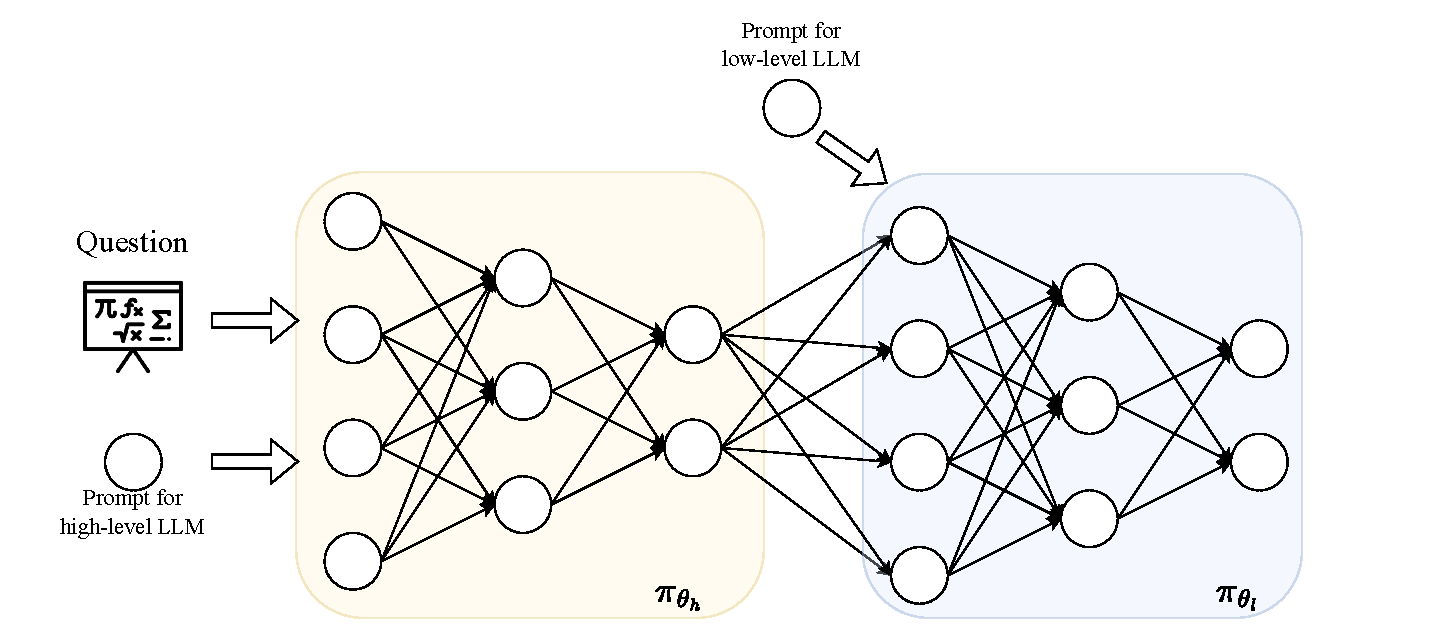
\includegraphics[width=1\linewidth]{figures/big_nn.pdf}
    \caption{
    Our method can be viewed as a combination of practical TRPO and block coordinate ascent, with the high and low-level models treated as distinct components within a larger neural network. Note that the figure does not represent the exact gradient back-propagation flow but rather highlights the key idea that we separate the high- and low-level models. This separation allows for the independent computation of gradients and the independent training of each model.
    % \zy{But there's not direct gradient can pass through low-level network to high-level network, unless we use tricks like gumble softmax for sequential outputs}
    }
    \label{fig:big_nn}
\end{figure}

We reuse the notations from Sec.~\ref{sec:method.reinforce_ma.it_train}, where $\mathbf{x}$ is task prompt, $\mathbf{y}$ is generated answer, $\mathbf{y}^*$ is ground-truth, $\mathbf{m}$ is metacognition on task solving, $\pi_{\theta_h}$ and $\pi_{\theta_l}$ are high- and low-level agents with parameters $\theta_h$ and $\theta_l$. We consider the joint hierarchical policy defined in Eq.~(\ref{eq:joint_policy}) and update the objective as in Eq.~(\ref{eq:combine_obj}).

To leverage existing RL and optimization convergence analysis methods, we treat the two models as components of a larger model, as illustrated in Fig.~\ref{fig:big_nn}. 
% We define a joint hierarchical policy with sequential decisions as follows:
% $$
% \pi(\theta_h, \theta_l) = \pi_l(\mathbf{y} \mid \mathbf{x}, \mathbf{m}\sim \pi_h(\mathbf{m}\mid\mathbf{x}; \theta_h); \theta_l),
% $$
% in which we use $\pi_h$ and $\pi_l$ for $\pi_{\theta_h}$ and $\pi_{\theta_l}$ for simplicity. Let $R(y, y^*)$ denote the 0/1 final correctness reward, which serves as the objective function $J(\theta_h, \theta_l)$ for the joint policy:
% $$
% J(\theta_h, \theta_l) = \mathbb{E}_{\mathbf{x}, \mathbf{y}^*} \mathbb{E}_{\mathbf{y}\sim \pi(\theta_h, \theta_l)} R(\mathbf{y}, \mathbf{y}*).
% $$
When updating one model, we treat the other model as part of a stationary environment. The gradients with respect to $\theta_h$ and $\theta_l$ are:
\begin{align*}
% &\textcolor{red}{\nabla_{\theta_h} J(\theta_h, \theta_l) = \mathbb{E}_{\mathbf{x}, \mathbf{y}^*} \sum_{\mathbf{y}\sim \pi(\theta_h, \theta_l)} \nabla_\mathbf{m}\pi_l(\mathbf{y} \mid \mathbf{x}, \mathbf{m}; \theta_h); \theta_l) \nabla_{\theta_h}\pi_h(\mathbf{m}\mid\mathbf{x}; \theta_h) R(\mathbf{y}, \mathbf{y}*)}, \\
&\nabla_{\theta_h} J(\theta_h, \theta_l) = \mathbb{E}_{\mathbf{x}, \mathbf{y}^*} \sum_{\mathbf{m}\sim \pi_h(\mathbf{m}\mid\mathbf{x}; \theta_h)} \nabla_{\theta_h}\pi_h(\mathbf{m}\mid\mathbf{x}; \theta_h) \left[\mathbb{E}_{\mathbf{y} \sim \pi_l(\mathbf{y} \mid \mathbf{x}, \mathbf{m})} R(\mathbf{y}, \mathbf{y}*)\right], \\
&\nabla_{\theta_l} J(\theta_h, \theta_l) = \mathbb{E}_{\mathbf{x}, \mathbf{y}^*} \sum_{\mathbf{y}\sim \pi(\theta_h, \theta_l)} \nabla_{\theta_l}\pi_l(\mathbf{y} \mid \mathbf{x}, \mathbf{m}; \theta_h); \theta_l) R(\mathbf{y}, \mathbf{y}*).
\end{align*}
We can compute the gradients with log trick and estimate $\mathbb{E}_{\mathbf{y} \sim \pi_l(\mathbf{y} \mid \mathbf{x}, \mathbf{m})} R(\mathbf{y}, \mathbf{y}*)$ with Monte Carlo method.

Equipped with the objective function and gradient computation, we update the models iteratively. Without loss of generality, we analyze the case where the high-level policy is updated first:
\begin{align*}
    &\theta_h^{(t+1)} = \arg\max_{\theta_h} J(\theta_h, \theta_l^{(t)}), \\
    &\theta_l^{(t+1)} = \arg\max_{\theta_l} J(\theta_h^{(t+1)}, \theta_l).
\end{align*}
Regarding the different regularizations $R_h$ and $R_l$ in Eqs.~(\ref{eq:rl.high}) and (\ref{eq:rl.low}) for the different policies, instead of directly integrating them into the loss function, we treat them as constraints, as done in Trust Region Policy Optimization (TRPO) \citep{DBLP:conf/icml/SchulmanLAJM15}. Note that when one policy is fixed, the other policy operates in a stationary decision process.

Based on the defined objective and update method, we apply TRPO and block coordinate ascent. First, recall that when updating a single policy, TRPO guarantees monotonic improvement by optimizing a lower bound. Specifically, let $\pi_{\text{old}}$ and $\pi$ represent the old and current policies, respectively. We define a surrogate objective as:
$$
L_{\pi_{\text{old}}}(\pi) = \mathbb{E}_{s\sim \pi_\text{old}, a\sim \pi_\text{old}}\left[ \frac{\pi(a|s)}{\pi_\text{old}(a|s)}A^{\pi_{\text{old}}} (s, a) \right],
$$
As shown by \citet{DBLP:conf/icml/SchulmanLAJM15}, the true objective of $\pi$ is lower-bounded by:
$$
J(\pi) \geq L_{\pi_{\text{old}}}(\pi) - C \cdot \max_s \operatorname{KL}[\pi_\text{old}(\cdot \mid s), \pi(\cdot \mid s)],
$$
for some constant $C$.
By optimizing the right-hand side of the above inequality, we are guaranteed to improve the performance of $\pi$. Therefore, for policies $\pi^t$ and $\pi^{t+1}$ obtained from iterations $t$ and $t+1$ using the TRPO method, we have:
$$
J(\pi^{t+1}) \geq J(\pi^t).
$$

Now, returning to our updating method, we treat the high- and low-level policies as two blocks of a single agent. The iterative update process can thus be viewed as a cyclic block coordinate ascent, where the two policies are updated in a fixed order. By updating each block using the TRPO method, and improving the surrogate objective within the KL constraint, each block update does not decrease $J$:
\begin{align*}
    &J(\theta_h^{t+1}, \theta_l^{t}) \geq J(\theta_h^{t}, \theta_l^{t}), \\
    &J(\theta_h^{t+1}, \theta_l^{t+1}) \geq J(\theta_h^{t+1}, \theta_l^{t}).
\end{align*}

Thus $J(\theta_h^{t+1}, \theta_l^{t+1}) \geq J(\theta_h^{t}, \theta_l^{t})$. This repeated coordinate maximization converges to a fixed point, where no single coordinate update can further improve $J(\theta_h, \theta_l)$.

Given the theoretical monotonic improvement with TRPO and block coordinate ascent, we adopt a practical version of TRPO in our experiments, specifically Proximal Policy Optimization (PPO) \citep{DBLP:journals/corr/SchulmanWDRK17} or GRPO \citep{shao2024deepseekmath}.



\subsection{Learning to reason from the perspective of Leader Follower Game } \label{sec:app_lfg}

% \zy{Add something about formulation}
% \yx{why do you add this formulation? we do not use these afterwards}
% We can formulate MAMRP as an extensive form game:
% \begin{equation}
%     G=\{\mathcal{N, A, H, Z},\chi, \rho, \sigma, u\},
% \end{equation}
% where $\mathcal{N}$ is a set of players, $\mathcal{A}$ is a set of actions spaces which is the natural language space for both players in our work, $\mathcal{H}$ is a set of non-terminal choices nodes, $\mathcal{Z}$ is a set of terminal nodes. $\chi$ is the action function, which assigns each choice node a set of possible actions from $\mathcal{A}$. $\rho$ is the player function which assigns each non-terminal node to a certain player that will make an action on it. $\sigma:\mathcal{H}\times\mathcal{A}\rightarrow \mathcal{H} \cup \mathcal{Z}$ is the transition function that describe the dynamics of the game. And $u=(u_1, \ldots, u_n), u_i:\mathcal{Z}\rightarrow \mathbb{R}$ is each player's reward and the end of the game.
% \zy{Is it necessary for us to model as extensive form game?}
% \yx{Just want to zhan keng}

Besides the loss function in the main part, we also propose to frame the problem as a leader-follower game. By analyzing the equilibria of the leader-follower game, we demonstrate that our framework inherently identifies the optimal sub-tasks aligned with the capabilities of the low-level model. This ensures that the high-level decisions are guided by the low-level model’s strengths, leading to more efficient and targeted task decomposition.
\subsubsection{Leader-follower game} \label{lfg}
The leader-follower game, also known as the Stackelberg game, models interaction between two agents with parametrized strategies $\boldsymbol{\theta} = (\boldsymbol{\theta}_1, \boldsymbol{\theta}_2)$ and differentiable objective functions $(\mathcal{L}_1, \mathcal{L}_2): \mathbb{R}^d \rightarrow \mathbb{R}$. In this framework, the leader announces its strategy first, and the follower observes this decision to respond optimally. This sequential structure enables the leader to anticipate the follower’s reaction and adjust its strategy accordingly. A Stackelberg equilibrium occurs when neither agent can unilaterally improve its objective. Denoting $\boldsymbol{\theta}_1$ as the leader’s strategy and $\boldsymbol{\theta}_2$ as the follower’s, the loss functions $\mathcal{L}_1$ and $\mathcal{L}_2$ are optimized with the following bi-level structure:
\begin{align*}
    \boldsymbol{\theta}_1^* = \argminvar_{\boldsymbol{\theta}_1} \mathcal{L}_1(\boldsymbol{\theta}, \boldsymbol{\theta}_2^*(\boldsymbol{\theta}_1)), \quad \boldsymbol{w}_2^*(\boldsymbol{\theta}_1) = \argminvar_{\boldsymbol{\theta}_2} \mathcal{L}_2(\boldsymbol{\theta}_1, \boldsymbol{\theta}_2).
\end{align*}

\citet{DBLP:journals/corr/abs-2108-12099} apply the leader-follower game to ensure checkable answers in a prover-verifier game (PVG). The objective is a verifier that is both complete (accepts all correct proofs from a verifier) and sound (rejects all incorrect proofs from a verifier). They analyze different scenarios where the verifier acts as the leader, the prover as the follower, and both announce strategies simultaneously, forming a Nash equilibrium. The study concludes that in verifier-led PVG, a Stackelberg equilibrium is both necessary and sufficient for achieving a sound and complete verifier, whereas in other configurations, a Stackelberg equilibrium is not necessary or sufficient for this outcome.

\subsubsection{Efficacy of LLM}
Because the high-level policy possesses strong generalization capabilities, it is impractical for it to exhaustively explore every potential sub-task for each question. Instead, it naturally focuses on tasks within a feasible range of difficulty, leveraging only a limited set of coarse planning actions. Rather than pinpointing perfectly tailored sub-tasks, the policy searches for general tasks of particular computational complexity, \ie, difficulty, that it can handle reliably.
Motivated by this perspective, we incorporate the concept of a reasoning boundary for large language models (LLMs) \citep{chen2024unlocking}. Intuitively, the reasoning boundary circumscribes the maximum difficulty of problems a model can solve at a desired accuracy level. Formally, for a model $\theta$, a task $t$, and a predefined threshold $A$, the reasoning boundary of $\theta$ represents the maximum problem difficulty $d$ that satisfies:
\begin{align*}
    \mathcal{B}_{Acc=A}(t|\theta)=\sup_d\{d|Acc(t|d,\theta)=A\}.
\end{align*}
where $d$ denotes the problem difficulty. By quantifying the difficulty level a model can reliably handle, the reasoning boundary provides a systematic way to align the high-level policy’s focus with the model’s actual capabilities, gauge the efficacy of the low-level policy, and determine the optimal strategy for solving the question.

\subsubsection{Leader-follower Game for LLM Reasoning}

Our goal is to find the high-level policy that searches for the sub-task sequence based on the efficacy of the low-level policy to solve the question. We design the loss functions as follows:
\begin{align*}
    & \mathcal{L}_h = \mathbb{E}_{(x, y)\sim p_D, t_{1:K}}\left[ -\log \pi_l(y_K \mid x, t_{1:K}, y_{1:K-1}) \right], \\
    & \mathcal{L}_l = \mathbb{E}_{x\sim p_D, t_{1:k}\sim \pi_h, \hat{y}_k \sim \pi_l} \left[ -r(y_k, \hat{y}_k \mid x, t_{1:k}, y_{1:k-1}) \right],
\end{align*}
where $r(y_k, \hat{y}_k \mid x, t_{1:k}, y_{1:k-1})$ represents the step reward for the correctness of $\hat{y}_k$ derived from the question $x$, the sub-task sequence $t_{1:k}$ from the high policy and prior intermediate answer $y_{1:k-1}$.
The loss functions can be interpreted as follows: the high-level policy is incentivized to find sub-tasks that lead to the correct answer based on the capabilities of the low-level policy, while the low-level policy is incentivized to enhance its instruction-following ability.

How to minimize the loss functions and whether such minimization leads to the desired results remain questions. To explore this, we consider a simplified case of our method, where the high-level policy plans the complete sub-task sequence at the beginning and the low-level executes the instruction in a single interaction. The corresponding parameterized policies are defined as $\pi_h((t_1, \dots, t_K) \mid x)$ and $\pi_l((\hat{y}_1, \dots, \hat{y}_K)\mid x, (t_1, \dots, t_K))$.
The corresponding loss functions are:
\begin{align} \label{eq:single_loss}
    & \mathcal{L}_h = \mathbb{E}_{(x, y)\sim p_D, t_{1:K}}\left[ -\log \pi_l(y_K \mid x, t_{1:K}) \right], \\
    & \mathcal{L}_l = \mathbb{E}_{x\sim p_D, t_{1:k}\sim \pi_h, \hat{y}_k \sim \pi_l} \left[ -r(y_k, \hat{y}_k \mid x, t_{1:k}, y_{1:k-1}) \right].
\end{align}
In this step, the high-level policy generates the entire sub-task sequence without relying on intermediate answers, while the low-level policy follows the sequence to produce answers for the sub-tasks. The low-level policy can still leverage prior intermediate answers to sequentially refine its responses.

To analyze the result agents by minimizing the loss functions, we adopt the completeness and soundness properties from the PVG framework for LLM reasoning. Specifically, if the high-level policy generates a sub-task sequence that is executable within the low-level policy’s capabilities, the problem must be solved (completeness). Conversely, if the sub-task sequence is incorrect or beyond the low-level policy’s capacity, the problem cannot be solved (soundness). To achieve this, we utilize the conclusion from \citet{DBLP:journals/corr/abs-2108-12099}, which positions the low-level policy as the leader and the high-level policy as the follower, equilibria guarantee the complete and sound low-level policy. 

When the high-level policy takes the lead, the low-level policy is forced to adapt to the specific strategy defined by the high-level policy, which can result in neither complete nor sound low-level policy. For example, if the high-level policy dictates that it will only generate sub-tasks involving addition and subtraction, the low-level policy is constrained to optimize only for these tasks. While they may reach an equilibrium, the low-level policy remains incomplete, and this limitation impacts both policies. In the case of the simultaneous PVG game, convergence to a Nash equilibrium is possible, but it is not sufficient for completeness and soundness. For instance, the low-level policy might disregard the high-level policy entirely (e.g., if the high-level provides incorrect instructions, but the low-level still performs correctly). This approach, however, is challenging to implement due to the significantly larger search space involved.

Furthermore, the loss functions we design ensure that, at a Stackelberg equilibrium, the high-level policy identifies sub-task sequences that the low-level policy can execute to solve the problem with the highest probability. With the low-level policy acting as the leader, it establishes its reasoning boundary for tasks. Based on the reasoning boundary, let $\theta_h$ and $\theta_l$ represent the policy parameters for the high-level and low-level policies, respectively. The probability that the low-level policy correctly solves the question is defined as:
\begin{align*}
    \pi_l(y_K \mid x, t_{1:K}) = \prod_{k=1}^K \text{Acc}(t_k \mid x, \theta_l),
\end{align*}
where we can compute the difficulty $d_k$ from $t_k$ and $x$.
where the difficulty $d_k$ can be derived from $t_k$ and $x$. The loss function in Eq.~(\ref{eq:single_loss}) ensures that the selected sub-tasks are optimal for the low-level policy.  Here we provide a theoretical condition under which the most efficient solution strategy can be identified, according to the efficacy of the LLM.

This approach can be viewed as a game between a high-level "prover" and a low-level "verifier". The verifier, representing the low-level policy, adheres the high-level policy’s instructions to validate its reasoning. Unlike the classic PVG setting, where the prover has ground-truth labels, the label of our high-level policy depends on the tunable low-level policy. This distinction, where the low-level policy (leader) is inherently more complex, contrasts with traditional PVG setups and adds complexity due to the interdependence between the high- and low-level policies.

By framing the problem-solving process as a leader-follower game, with the low-level policy designated as the leader, we can construct a bi-level optimization problem to identify an equilibrium. Following the formulation in Sec.~\ref{lfg}, the problem is expressed as:
\begin{align*}
    \theta_l^* = \argmin_{\theta_l} \mathcal{L}_l(\theta_h^*(\theta_l), \theta_l) \quad \theta_h^*(\theta_l) = \argmin_{\theta_l}\mathcal{L}_h(\theta_h, \theta_l).
\end{align*}
Then we can apply bi-level optimization techniques. 
% Here we adopt the optimization method from \citet{DBLP:journals/siamjo/HongWWY23}

\section{Training Details}
\label{app:exp_setting}

\subsection{Single-turn ReMA}
\label{app:exp_setting.single_turn_rema}
We refer to Appendix~\ref{app:prompts} for prompts we use during training.
We implement the training pipeline with OpenRLHF \citep{hu2024openrlhf} which is a highly efficient codebase and is easy to scale up.
We select REINFORCE++ to save resources and for efficient training. All experiments are conducted in a node of 8 NVIDIA A100 GPUs. We use bf16, Zero2, Flash-Attention and gradient checkpointing to run our experiments.

During rollout, we set temperature=1.0, top\_p=1.0, top\_k=-1, and use vLLM for inference acceleration. We set the max generation length to be 2048 and, the rollout batch size to be 1000. The number of samples per prompt is 4. During training, we use Adam Optimizer with a learning rate of 5e-7. We set the mini-batch size to be 500, and the clip ratio to be 0.2. 
Other hyperparameters, such as KL coefficients and the number of training episodes, were carefully tuned based on validation set performance to ensure robust and reliable results. To align with the hyperparameter in OpenRLHF, we use \#Training Episode as the number of reinforcement learning epoch on the entire dataset.

In \method, during prompt filtering of the high-level model, the high-level agent first samples 10 candidates for each question with t=1.0, and for each output the low-level agents sample 1 solution with t=0.0, then we select questions of success rate between $[\varepsilon_{\min}, \varepsilon_{\max}]$. And for the low-level agent's prompt filtering, the high-level agent first samples 1 candidate for each question with t=0.0, and for each output the low-level agents sample 10 solutions with t=1.0, then we select questions of success rate between $[\varepsilon_{\min}, \varepsilon_{\max}]$ and use the high-level agent to sample 4 meta-thoughts with t=1.0 as the input.
\subsubsection{Supervised fine-tuning data collection} 
\label{app:exp_setting.single_turn_rema.sft_data}
For experiments in Sec.~\ref{sec:exp.low_rl}, we collect expert data to enhance the reasoning pattern, \ie \textit{RL from SFT}. Specifically, we collect demonstration data from GPT-4o Mini on MATH training dataset (7.5k problems) \citet{hendrycks2021measuring} and use it to fine-tune the LLMs. The data generation follows these steps: First, we prompt GPT-4o Mini to produce metacognitive reasoning for high-level model training. Specifically, we use different prompts to instruct it to rewrite and decompose a given question without providing a final answer. We collect metacognitive reasoning using two predefined actions, ``rewrite” and ``decompose”, which align with human approaches to complex problem-solving while preserving answer diversity. Next, we use the generated instructions to prompt GPT-4o Mini to follow the metacognitive steps and solve the question, obtaining SFT data for low-level policy training. Below, we present the prompts used for both high-level and low-level models.
% \yx{we use JSON format...we need to make up something why we do this.}
Prompts can be found in Appendix~\ref{app:prompts.single_turn_rema.json_data}.



\subsubsection{Dataset Curation of RewardBench970}
\label{app:exp_setting.single_turn_rema.rewardbench970}
\begin{table}[h!]
    \centering
    \caption{Performance on LLM-as-a-Judge benchmarks, trained on dataset under the loose setting. The two-agent workflow in \method }
    \label{tab:exp.abl.data_split.laaj}
    \begin{tabular}{c||c|cccc}
        
        \toprule
        \textbf{Model} & \textbf{Benchmark} & \makecell{\textbf{VRP}\\(CoT)} & \textbf{VRP$_\text{RL}$} & \textbf{MRP$_\text{RL}$ }& \makecell{\textbf{\method}\\(Ours)} \\ 
        \toprule
        \multirow{3}{*}{\textbf{\makecell{Llama3.1\\-8B\\-Instruct}}}
        & \cellcolor{InDist} RewardBench970 & 71.24 & 81.86 (\textcolor{red}{+10.62}) & 80.41 (\textcolor{red}{+9.17}) & \textbf{86.29 (\textcolor{red}{+15.05})} \\
& \cellcolor{OutDist} JudgeBench & 51.77 & 51.45 (\textcolor{DarkGreen}{-0.32}) & 50.65 (\textcolor{DarkGreen}{-1.12}) & \textbf{53.71 (\textcolor{red}{+1.94})} \\
\cmidrule{2-6}
& Average & 61.51 & 66.65 (\textcolor{red}{+5.14}) & 65.53 (\textcolor{red}{+4.02}) & \textbf{70.00 (\textcolor{red}{+8.49})} \\
        \toprule        
        \multirow{3}{*}{\textbf{\makecell{Qwen2.5\\-7B\\-Instruct}}}
        & \cellcolor{InDist} RewardBench970 & 86.49 & 87.22 (\textcolor{red}{+0.73}) & 80.31 (\textcolor{DarkGreen}{-6.18}) & \textbf{90.72 (\textcolor{red}{+4.23})} \\
& \cellcolor{OutDist} JudgeBench & 58.39 & 54.84 (\textcolor{DarkGreen}{-3.55}) & 55.81 (\textcolor{DarkGreen}{-2.58}) & \textbf{58.71 (\textcolor{red}{+0.32})} \\
\cmidrule{2-6}
& Average & 72.44 & 71.03 (\textcolor{DarkGreen}{-1.41}) & 68.06 (\textcolor{DarkGreen}{-4.38}) & \textbf{74.72 (\textcolor{red}{+2.28})} \\
        \bottomrule
    \end{tabular}
\end{table}
We process the original dataset in RewardBench by splitting it into a training set containing 5,000 tuples of (instruction, response A, response B) and a test set with the remaining 970 tuples.

To ensure a meaningful dataset split, we validate two separation strategies:
\begin{itemize}
\item Loose setting: We only ensure that there is no direct overlap of tuples between the training and test sets.
\item Strict setting: We further enforce that no instruction appears in both the training and test sets. The results for this setting are presented in the main results (Table~\ref{tab:exp_main.laaj}).
\end{itemize}
Additionally, since the original RewardBench data originates from different subsets, we ensure that all original subsets are evenly represented in both the training and test sets.

Table~\ref{tab:exp.abl.data_split.laaj} reports the learning performance of various methods under the loose dataset split setting.
Compared to the results in Table~\ref{tab:exp_main.laaj}, \method~significantly outperforms other RL tuning baselines across all models, particularly on out-of-distribution (OOD) benchmarks. \textbf{The consistent improvements on OOD datasets of these two settings suggest that \method~enhances meta-thinking ability, resulting in better generalization across diverse task distributions.}



\subsubsection{Training on MATH}
\label{app:exp_setting.single_turn_rema.math}
\paragraph{VRP}
For Llama3-8B-Instruct, Llama3.1-8B-Instruct, and Qwen2.5-7B-Instruct, we all use a KL coefficient of 1e-2, and for \#Training Episode, we use 12,6,6 for these 3 models respectively. For Llama3-8B-Instruct, we set the learning rate of 2e-7 for stable training.
\paragraph{MRP}
For Llama3-8B-Instruct, Llama3.1-8B-Instruct, and Qwen2.5-7B-Instruct, we all use a KL coefficient of 1e-2, and for \#Training Episode, we use 10,6,6 for these 3 models respectively. 
\paragraph{MAMRP}
We use $\varepsilon_{\min}=0.2, \varepsilon_{\max}=0.8$ for prompt filtering.
We use the same \#Training Episode=4 for all models, and for \#Update Iteration, we use 3 for Llama3-8B-Instruct and Llama3.1-8B-Instruct, 10 for Qwen2.5-7B-Instruct. And we set the KL coefficient to be 1e-2 for all the 3 models.

\subsubsection{Training on Reward Bench}
\label{app:exp_setting.single_turn_rema.reward_bench}
\paragraph{VRP}
For Llama3.1-8B-Instruct, and Qwen2.5-7B-Instruct, we all use a KL coefficient of 1e-2, and for \#Training Episode, we use 4,6 for these 2 models respectively.
\paragraph{MRP}
For Llama3.1-8B-Instruct, and Qwen2.5-7B-Instruct, we all use a KL coefficient of 1e-2, and for \#Training Episode, we use 4,6 for these 2 models respectively.
\paragraph{MAMRP}
We set \#Update Iteration=1 for all models. We set the KL coefficient to be 1e-2 for Llama3.1-8B-Instruct and 1e-2 for Qwen2.5-7B-Instruct all models.
For Llama3.1-8B-Instruct, we use $\varepsilon_{\min}=0.2, \varepsilon_{\max}=0.8$ for prompt filtering and we use \#Training Episode of 2 during training.
For Llama3.1-8B-Instruct, we use $\varepsilon_{\min}=0.1, \varepsilon_{\max}=0.9$ for prompt filtering and we use \#Training Episode of 1 during training.

\subsection{Multi-turn ReMA}
\label{app:exp_setting.multi_turn_rema}
We refer to Appendix~\ref{app:prompts} for prompts we use during training. We implement a multi-turn ReMA training pipeline with VeRL \citep{sheng2024hybridflow} since it's easier to implement complex training pipeline with a single centralized controller. Similar to OpenRLHF, VeRL is also a highly efficient and scalable codebase for further development.

For the multi-turn ReMA rollout, we use parameter sharing and simultaneous update by default. In details, we maintain two message lists with the system prompt of meta-thinking agent and reasoning agent respectively. During rollout, each agent act as `assistant' in its own message list and the other agent act as `user'.
We use three hyperparameters to control the rollout length: 
(1) `\texttt{max\_num\_turns}': the maximum number of turns for each trajectory.
(2) `\texttt{max\_response\_length}': the maximum number of tokens for each turn's response.
(3) `\texttt{max\_prompt\_length}': the maximum number of tokens for each trajectory.

During training, we apply the collected message list to Qwen2.5-7B's chat template and build loss masks in order to compute the loss for all turns of one trajectory (message list).

Morever, for multi-turn ReMA rollout, unlike single agent single turn rollout, we need to carefully design the termination logic. Basically, \textbf{we let the meta-thinking agent automatically decides when to finish the solving procedure}, we use a special tag `\texttt{[FINISH]}' to indicate the end of the solving procedure. After we detect this tag, we will terminate trajectory after the reasoning agent generates its output.

We also design other termination conditions to ensure the quality of the generated trajectories. If the last agent's response is too long, we will terminate the whole trajectory and setting the reward to 0.
We also introduce a different version of format reward: we give a reward of 1.0 only if the reasoning agent's last turn response is correct and the meta-thinking agent's last turn response include `\texttt{[FINISH]}'.
We use \texttt{math\_verify} as the default verifier.

\subsubsection{SFT data collection of multi-turn MAMRP}
\label{app:exp_setting.multi_turn_rema.sft_data}
We use GPT-4o to translate 817 samples in LIMO \citep{ye2025limo} by prompting it to wrap each sentence with meta-thinking and reasoning tags.
We use a temperature of 0. After filtering, we get 800 conversations for training.
The prompt can be found in Appendix~\ref{app:prompts.multi_turn_rema.sft_data}.
For supervised finetuning, we use LlamaFactory as the codebase and train the model for 3 epochs with a learning rate of 1e-5, consine learning rate scheduler, and batch size of 8. Use DeepSpeed Zero2 for distributed training.


\subsubsection{Training on MATH}
\label{app:exp_setting.multi_turn_rema.math}
For training of multi-turn \method~on MATH, we use GRPO~\citep{shao2024deepseekmath} as the default learning algorithm.
We refer to Appendix~\ref{app:prompts.multi_turn_rema.math} for prompts.
For experiment in Sec~\ref{sec:exp.multiturn}, we use sample 128 prompts, each with 16 trajectories. During training, we drop the KL loss term to improve the numerical stability. We use a learning rate of 1e-6, bfloat16 precision, FSDP backend for distributed training. 
We split the rollout data into 4 mini-batches for update. For the sake of numerical stability, we do pre-clip before computing the exponential of \texttt{log\_prob} for a upperbound of 3.0.

For the main result in Fig~\ref{fig:multi_turn_main}, we test different rollout configurations with a \texttt{max\_prompt\_length} of 4096, training for 500 steps. We use 32 NVIDIA A800 GPUs, the longest training cost about 40 hours due to large scale validation per 10 steps.

For the ablation results in Fig~\ref{fig:multi_turn_ablation}, we use a tiny subset of MATH Level 3-5, training for 300 steps. Specifically, we sample 19 questions for every single type (133 instances in total). We use 8 NVIDIA A800 GPUs, the training cost about 30 hours

We test different rollout configurations:\\
(1) \texttt{max\_num\_turns=30}, \texttt{max\_response\_length=256}, \texttt{max\_prompt\_length=4096}
(2) \texttt{max\_num\_turns=30}, \texttt{max\_response\_length=1024}, \texttt{max\_prompt\_length=3072}

And for the experiment of separate parameter in multi-turn \method, we iteratively train each agent with the same configuration as above, but with a switch interval of 10 steps, starting from the meta-thinking agent.


\section{Other Experiments}
\label{app:other_exp}
\subsection{Reward functions shape cross-agent behaviors}
\label{exp:reward_design}
We also investigate the impact of different reward function designs on \method's behavior.  
In addition to the base reward setting described in Appendix~\ref{app:reward_design}, we evaluate a consistency-based reward function using Qwen2.5-7B-Instruct.  
This reward function is designed to encourage the high-level agent to generate more detailed guidance.  
Indeed, we observe that the high-level agent trained in this manner produces more detailed solution steps compared to the one trained with the basic correctness format reward.  
However, we also find that this approach often leads to jailbreak behavior, where the high-level agent tends to include the final answer within its output, compromising the intended hierarchical reasoning process.  

Furthermore, we discover an interesting evolution of a pattern during training: although our experimental setup is designed for the high-level agent to provide a solution plan while the lower-level agent executes it, we find that under the consistency-based reward, the lower-level agent significantly increases its attempt of verification rather than straightforward execution.
We observed a certain sentence commonly appearing in the low-level agent's responses:  
\textit{``Let's go through the solution step by step to ensure clarity and correctness."}
To quantify this effect, we track the frequency of it.  
We analyze this pattern across all mathematical test sets, sampling eight completions per question at a temperature of 0.7.  
%Our results show that this phrase appears \textbf{30 times more frequently}\hj{maybe a fancy name like 'aha moment' rather than the simple 'this phrase'} in the model trained with the consistency-based reward compared to the one trained with the base reward.
Our empirical results have identified a {\bf 30x increase} of such self-verifying patterns in the model trained with the consistency-based reward compared to the one trained with the base reward.
Moreover, we also observe additional variations of this pattern, e.g.
\textit{``Let's carefully re-evaluate the problem and solution to ensure accuracy and clarity."}  
These phrases indicate that the low-level agent is actively exploring to verify the detailed response provided by the high-level agent.

This suggests that (1) meta-thinking can not only emerge and be reinforced in the high-level agent but also in the low-level agent. During reinforcement learning (RL) training, the two agents develop \textbf{a novel problem-solving pattern} characterized by a \textbf{role reversal}. (2) \textbf{Consistency-based rewards promote a more self-corrective approach at the lower level}, potentially disrupting the intended separation of roles between planning and execution. For a detailed case study, refer to Appendix~\ref{app:qualative_results.case_study}.

\subsection{Detailed Training Curves on Different Datasets of Multi-turn \method}
\label{app:exp_setting.multi_turn_rema.detailed_training_curves}
We show the detailed training curves of the multi-turn \method~on different datasets in Fig.~\ref{fig:detailed_training_curves_2x4}.
\begin{figure}[h!]
    \centering
    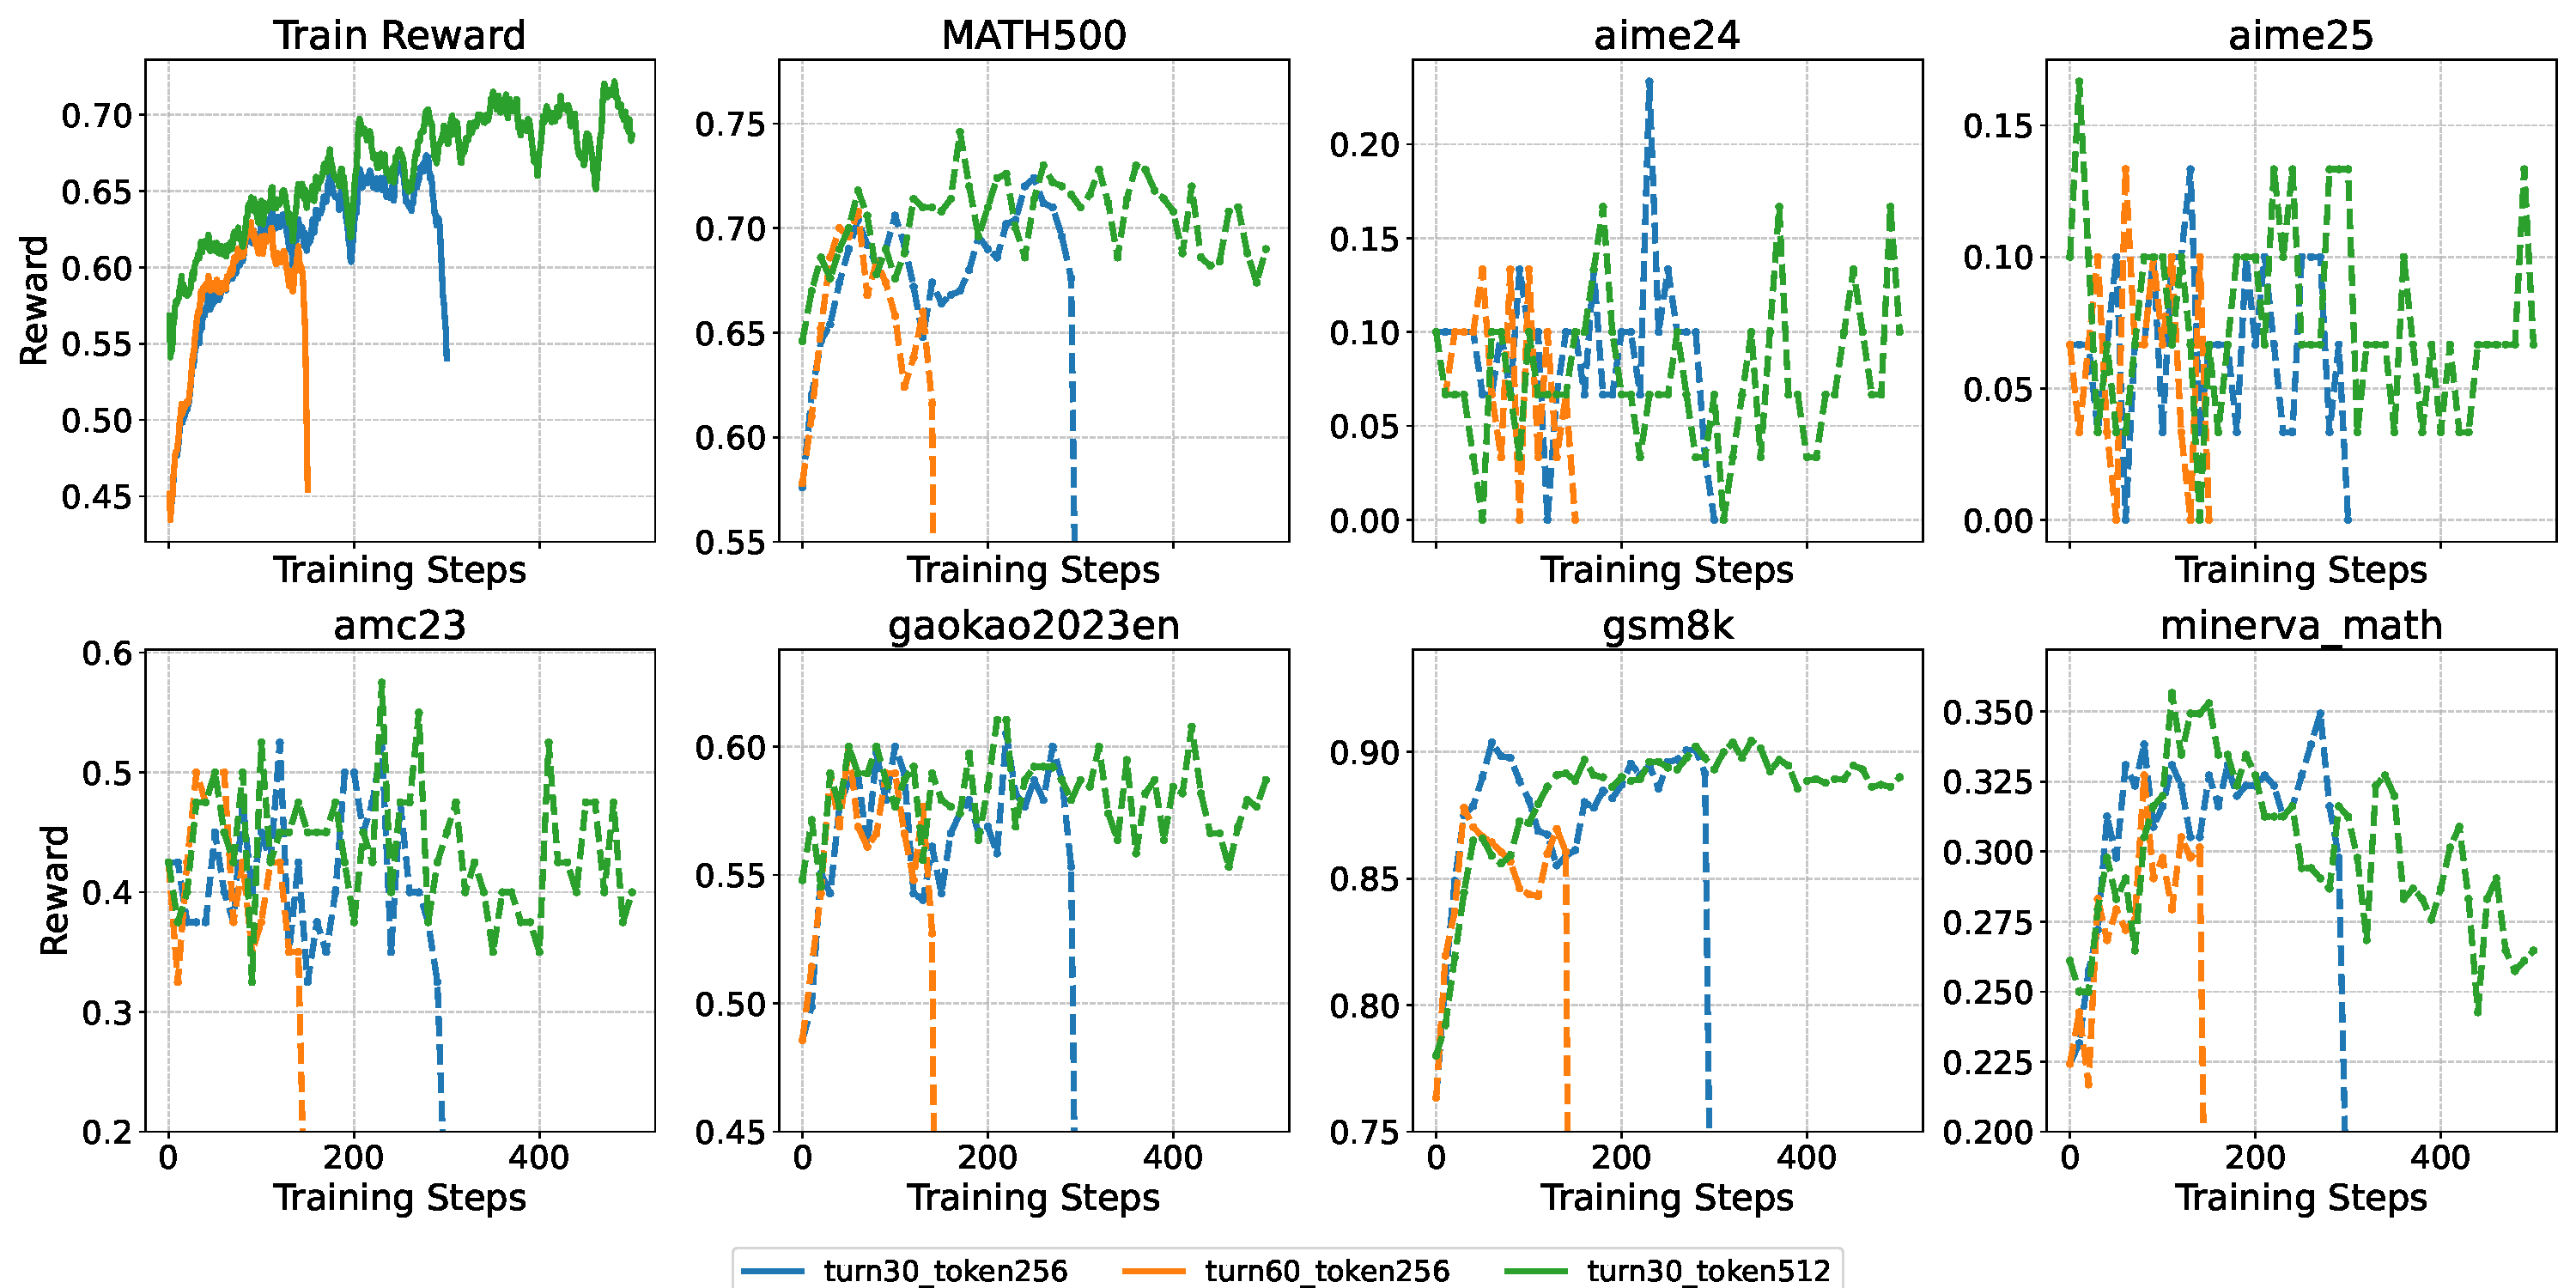
\includegraphics[width=1.0\linewidth]{figures/multi_turn/multi_turn_main_2x4.pdf}
    \caption{Detailed Training Curves on Different Datasets of Multi-turn \method}
    \label{fig:detailed_training_curves_2x4}
\end{figure}

\section{Qualitative Results}
\label{app:qualitative_results}

\subsection{High-level policy finds better plans}
\label{app:qualitative_results.high_level_better}
Here is an example of how a high-level policy alters the solving method of an LLM, increasing the likelihood of providing correct answers. 
As we can see from the following example, without the high-level policy, the LLM counts all integer coordinates, including those on the boundary, and then subtracts the boundary coordinates. In contrast, the high-level policy identifies a better approach, directly instructing the LLM to count only the coordinates strictly inside the boundary.

% \paragraph{Question:}\leavevmode \newline
% Consider the rectangular region with the following points as vertices: $$(5,4), (-5,4), (-5,-4), (5,-4).$$ How many points with integer coordinates will be strictly in the interior of this rectangular region?

% \paragraph{Output without high-level planning tends to solve this question in a less optimal way, often leading to a wrong answer:}\leavevmode \newline
% To determine how many points with integer coordinates will be strictly in the interior of the rectangular region with vertices at \((5, 4)\), \((-5, 4)\), \((-5, -4)\), and \((5, -4)\), we will follow these steps:\\1. Identify the dimensions of the rectangle:   - The width of the rectangle can be calculated as the distance between the x-coordinates of the vertices. The x-coordinates are \(-5\) and \(5\).   \[   \text{Width} = 5 - (-5) = 10   \]   - The height of the rectangle can be calculated as the distance between the y-coordinates of the vertices. The y-coordinates are \(4\) and \(-4\).   \[   \text{Height} = 4 - (-4) = 8   \]2. Calculate the total number of integer points:   - The total number of integer points in the rectangle (including the boundary) can be calculated by considering the range of x and y values:     - The x-values range from \(-5\) to \(5\), giving us \(11\) integer values (\(-5, -4, -3, -2, -1, 0, 1, 2, 3, 4, 5\)).     - The y-values range from \(-4\) to \(4\), giving us \(9\) integer values (\(-4, -3, -2, -1, 0, 1, 2, 3, 4\)).   - The total number of points in the rectangle (including the boundary) is:     \[     \text{Total points} = 11 \times 9 = 99     \]3. Calculate the number of points on the boundary:   - The boundary consists of the four sides of the rectangle.   - The top and bottom sides (y = 4 and y = -4) each have \(11\) integer points (from \(-5\) to \(5\)).   - The left and right sides (x = 5 and x = -5) each have \(9\) integer points (from \(-4\) to \(4\)).   - Therefore, the total number of points on the boundary is:   \[   \text{Boundary points} = 2 \times 11 + 2 \times 9 = 22 + 18 = 40   \]4. Calculate the number of strictly interior points:   - To find the number of points strictly in the interior, we subtract the points on the boundary from the total number of points:     \[     \text{Interior points} = \text{Total points} - \text{Boundary points} = 99 - 40 = 59     \]Thus, the number of points with integer coordinates that will be strictly in the interior of this rectangular region is \(\boxed{59}\)."

% \paragraph{Answer with high-level planning identifies the optimal sub-tasks for the LLM to solve, increasing the chance of answering the question correctly:}\leavevmode \newline
% \textbf{High-level policy planning}: First, identify the boundaries of the rectangular region. Then, determine the integer coordinates that lie strictly within these boundaries. Finally, count the number of such points. \newline
% \textbf{Low-level policy reasoning following the high-policy plan}: To solve the problem, we will follow the steps outlined in the instructions.

% Step 1: Identify the boundaries of the rectangular region. The vertices of the rectangular region are:- \((5, 4)\)- \((-5, 4)\)- \((-5, -4)\)- \((5, -4)\)From these vertices, we can determine the boundaries:- The left boundary is \(x = -5\).- The right boundary is \(x = 5\).- The bottom boundary is \(y = -4\).- The top boundary is \(y = 4\).

% Step 2: Determine the integer coordinates that lie strictly within these boundaries. For a point \((x, y)\) to be strictly inside the rectangle, it must satisfy:- \(-5 < x < 5\)- \(-4 < y < 4\)

% Step 3: Count the integer coordinates that satisfy these conditions. Now, we will find the integer values for \(x\) and \(y\) that fall within these boundaries. For \(x\):- The integer values that satisfy \(-5 < x < 5\) are:  \(-4, -3, -2, -1, 0, 1, 2, 3, 4\)- This gives us 9 possible integer values. For \(y\):- The integer values that satisfy \(-4 < y < 4\) are:  \(-3, -2, -1, 0, 1, 2, 3\). This gives us 7 possible integer values.

% Step 4: Calculate the total number of points. Now, we multiply the number of possible integer values for \(x\) by the number of possible integer values for \(y\):\[\text{Total points} = 9 \times 7 = 63\]Finally, the number of points with integer coordinates that lie strictly in the interior of the rectangular region is \(\boxed{63}\).
\begin{figure}[h!]
    \centering
    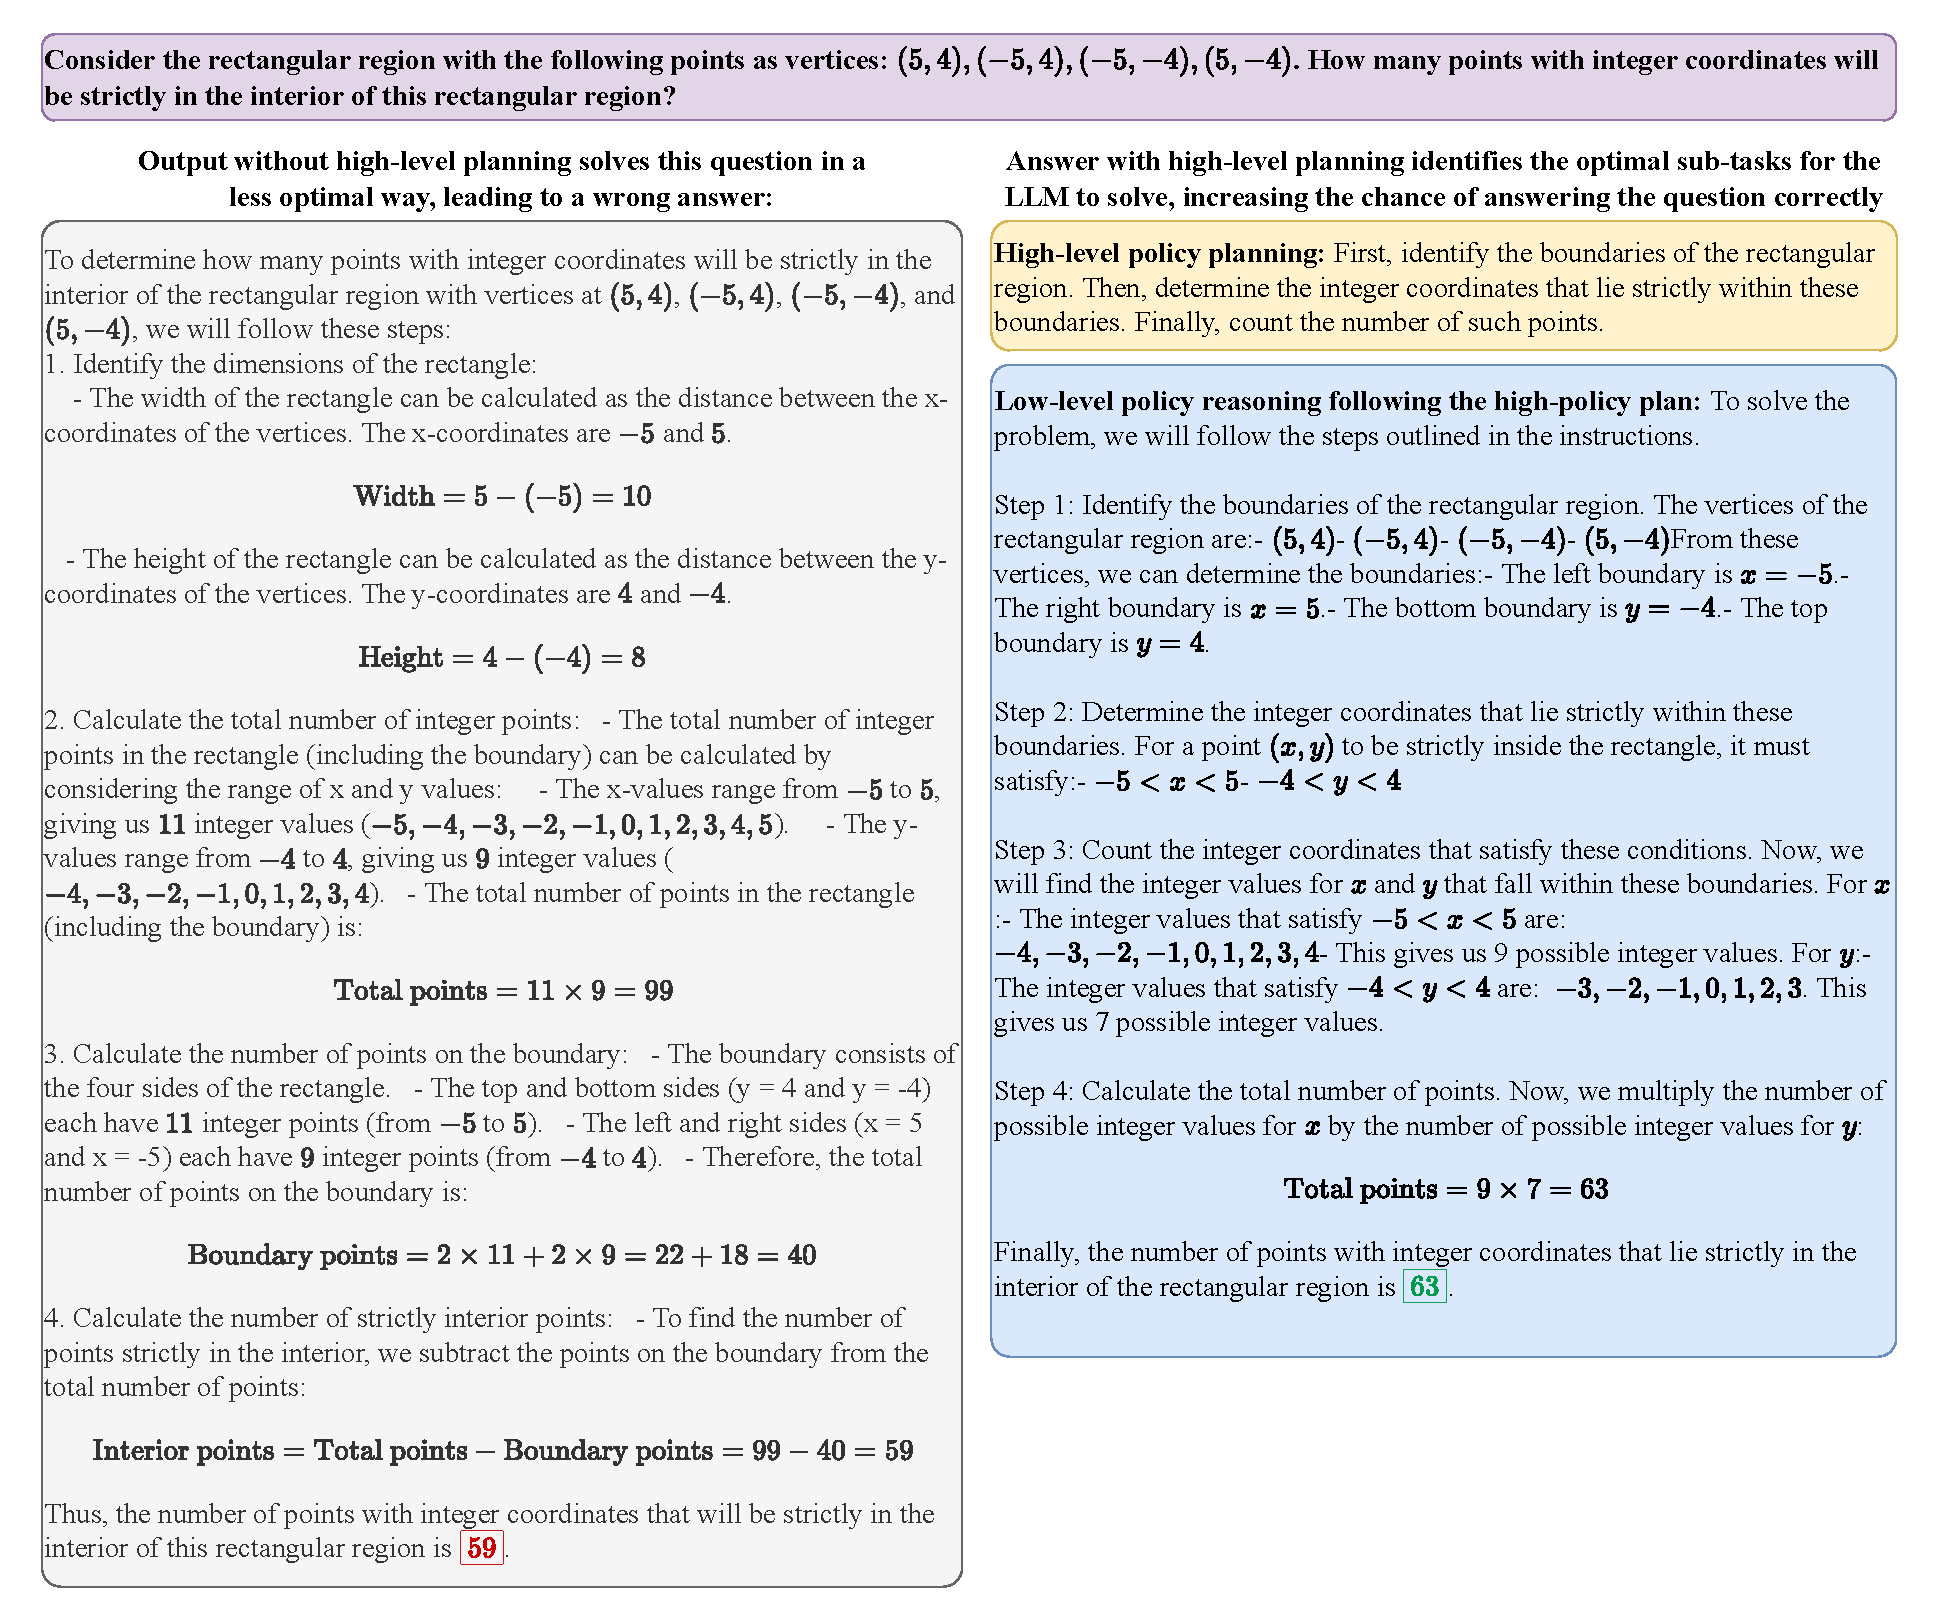
\includegraphics[width=1.0\linewidth]{figures/another_case_study.pdf}
    \caption{Case Study comparing with and without high-level metacognition results.}
    \label{fig:another_case_study}
\end{figure}



\subsection{Case study for Experiments in Section~\ref{exp:reward_design}}
Fig.~\ref{fig:qualative_results.reward_design.case_study1} and Fig.~\ref{fig:qualative_results.reward_design.case_study2} show an case study of experiments in Sec.~\ref{exp:reward_design}.

Although both agents are prompted with the same instructions as in our main results, the consistency reward of the high-level agent significantly alters the learning dynamics. As illustrated in Fig.~\ref{fig:qualative_results.reward_design.case_study1}, the high-level agent generates detailed solution attempts rather than a strategic plan. Consequently, the low-level agent evolves to verify the high-level agent’s solutions. This suggests that, during reinforcement learning (RL) training, the two agents develop \textbf{a novel problem-solving pattern} characterized by a \textbf{role reversal}, where one agent generates an answer while the other verifies it.

\label{app:qualative_results.case_study}
\begin{figure}[h!]
    \centering
    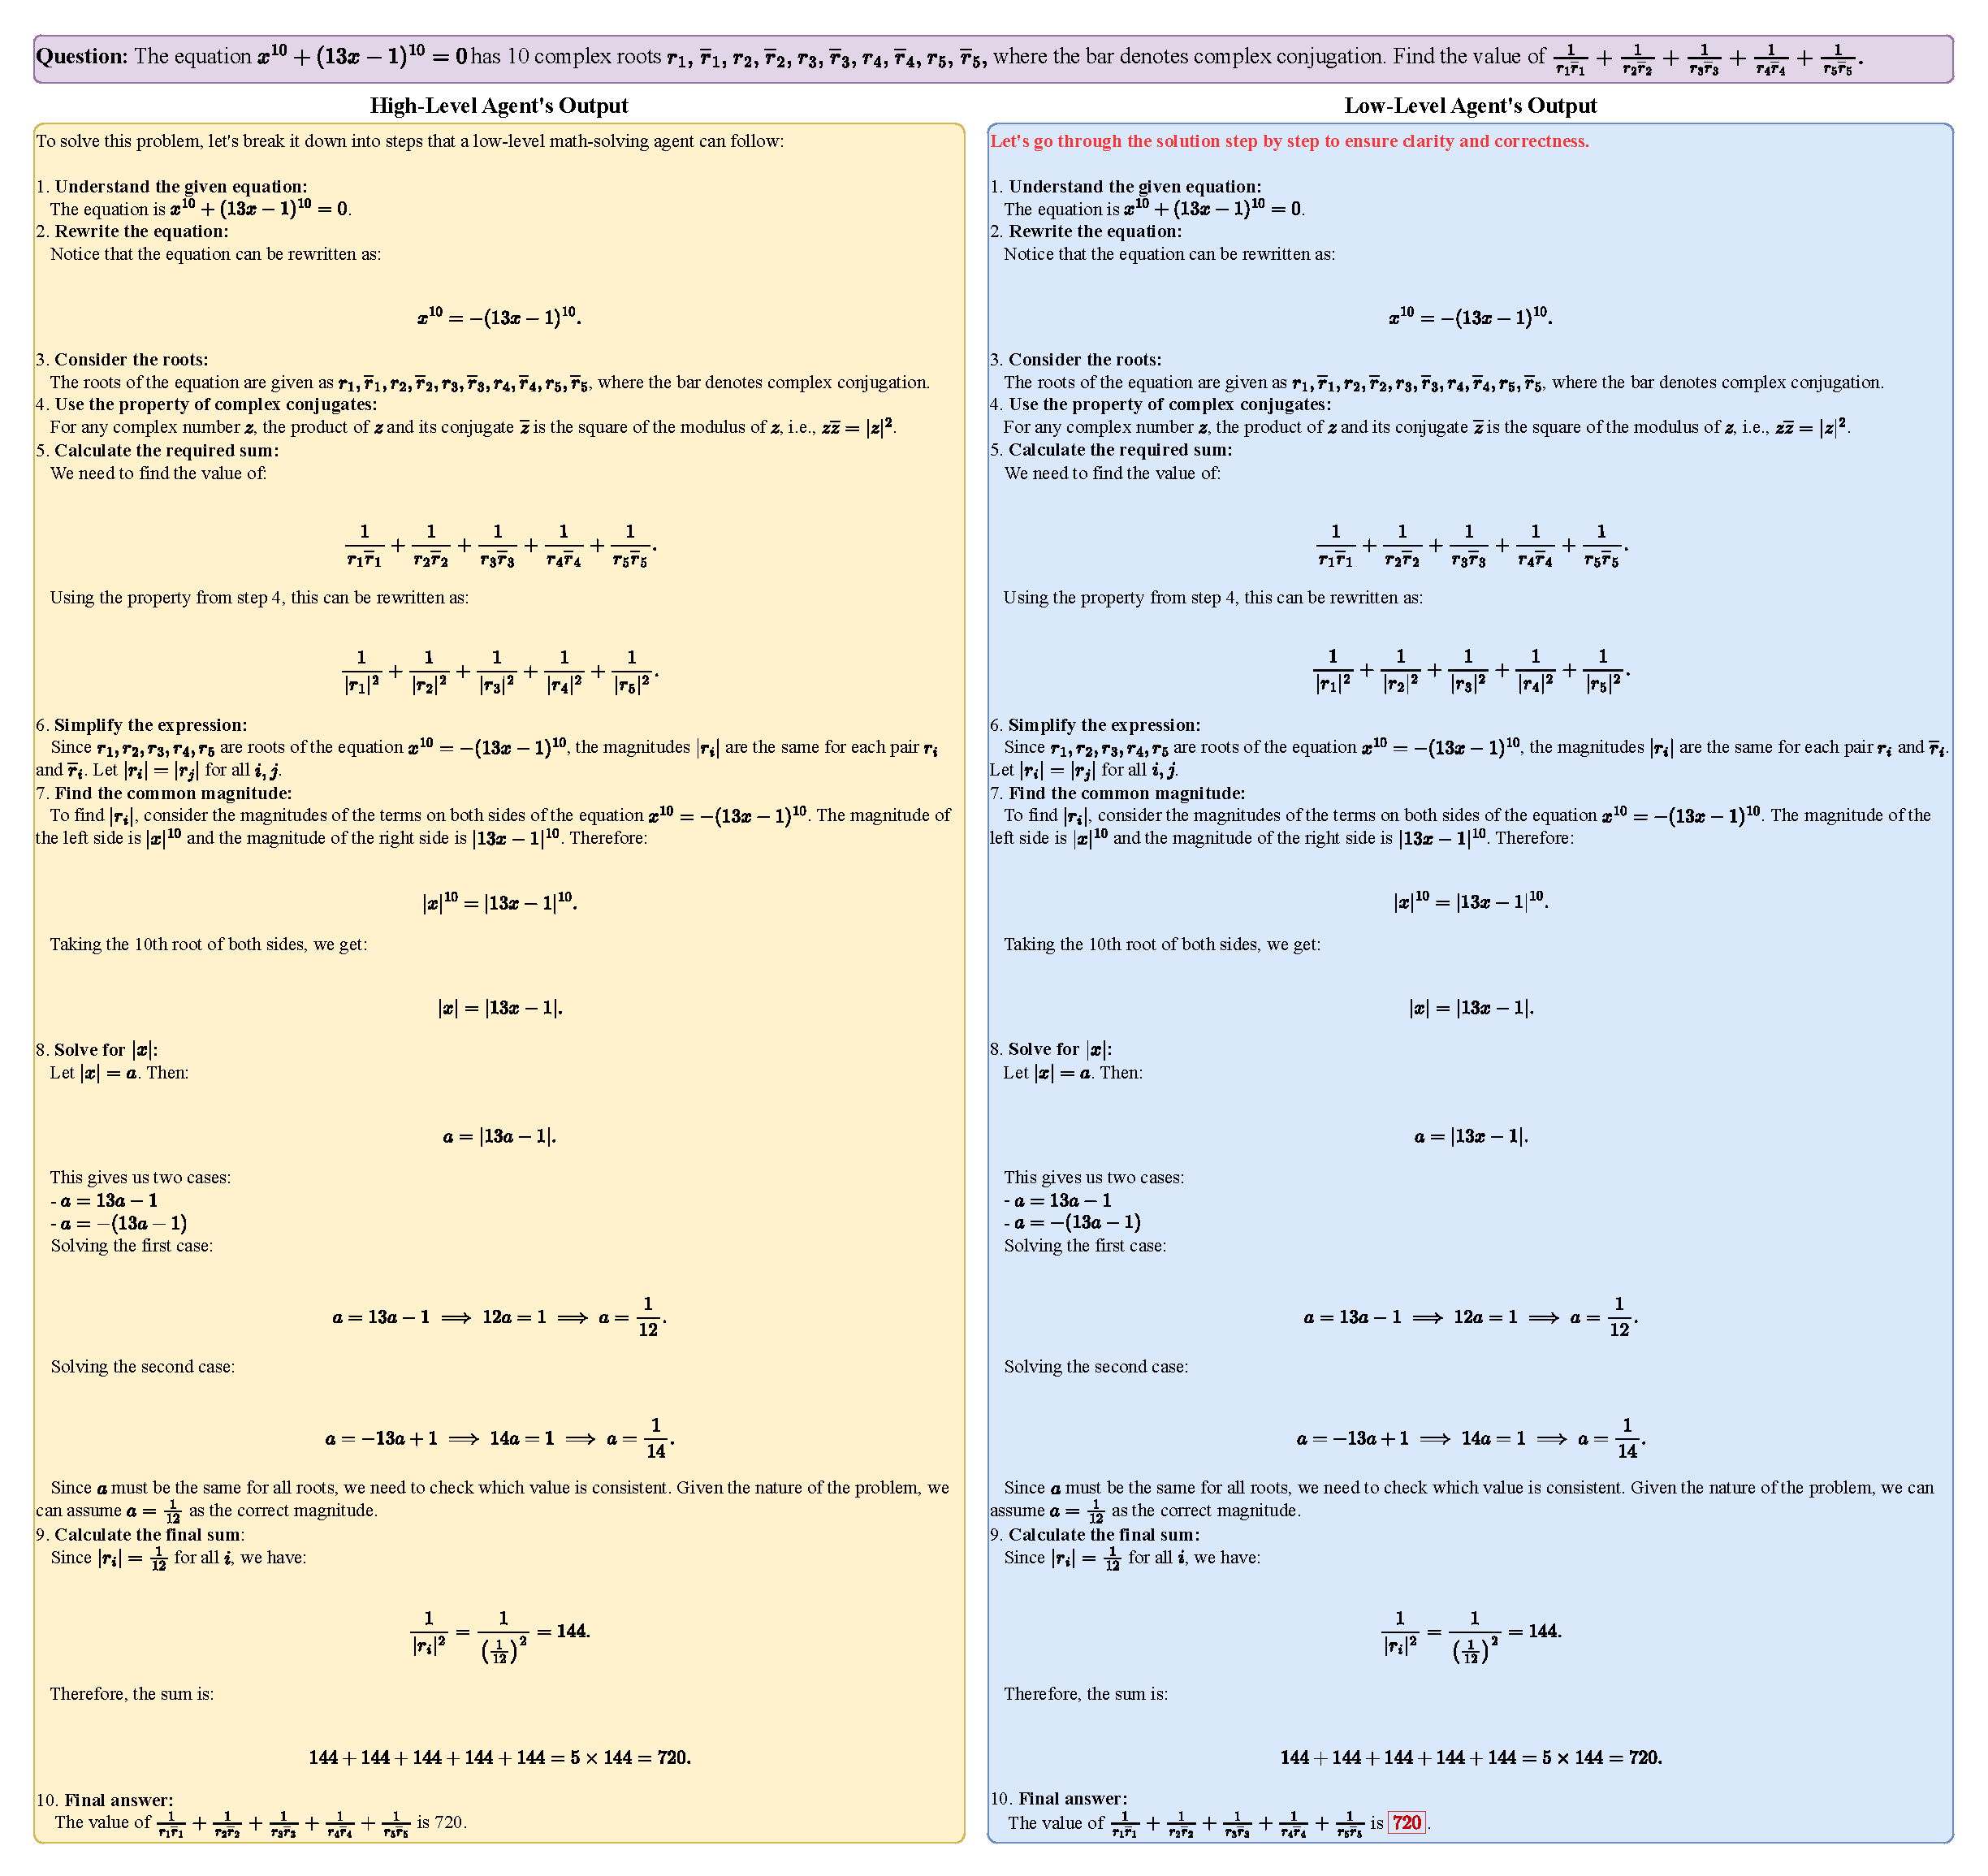
\includegraphics[width=1.0\linewidth]{figures/reward_design_case_studies/exp_reward_design_case_study1.pdf}
    \caption{Case Study for consistency reward of high-level agent}
    \label{fig:qualative_results.reward_design.case_study1}
\end{figure}

\begin{figure}[h!]
    \centering
    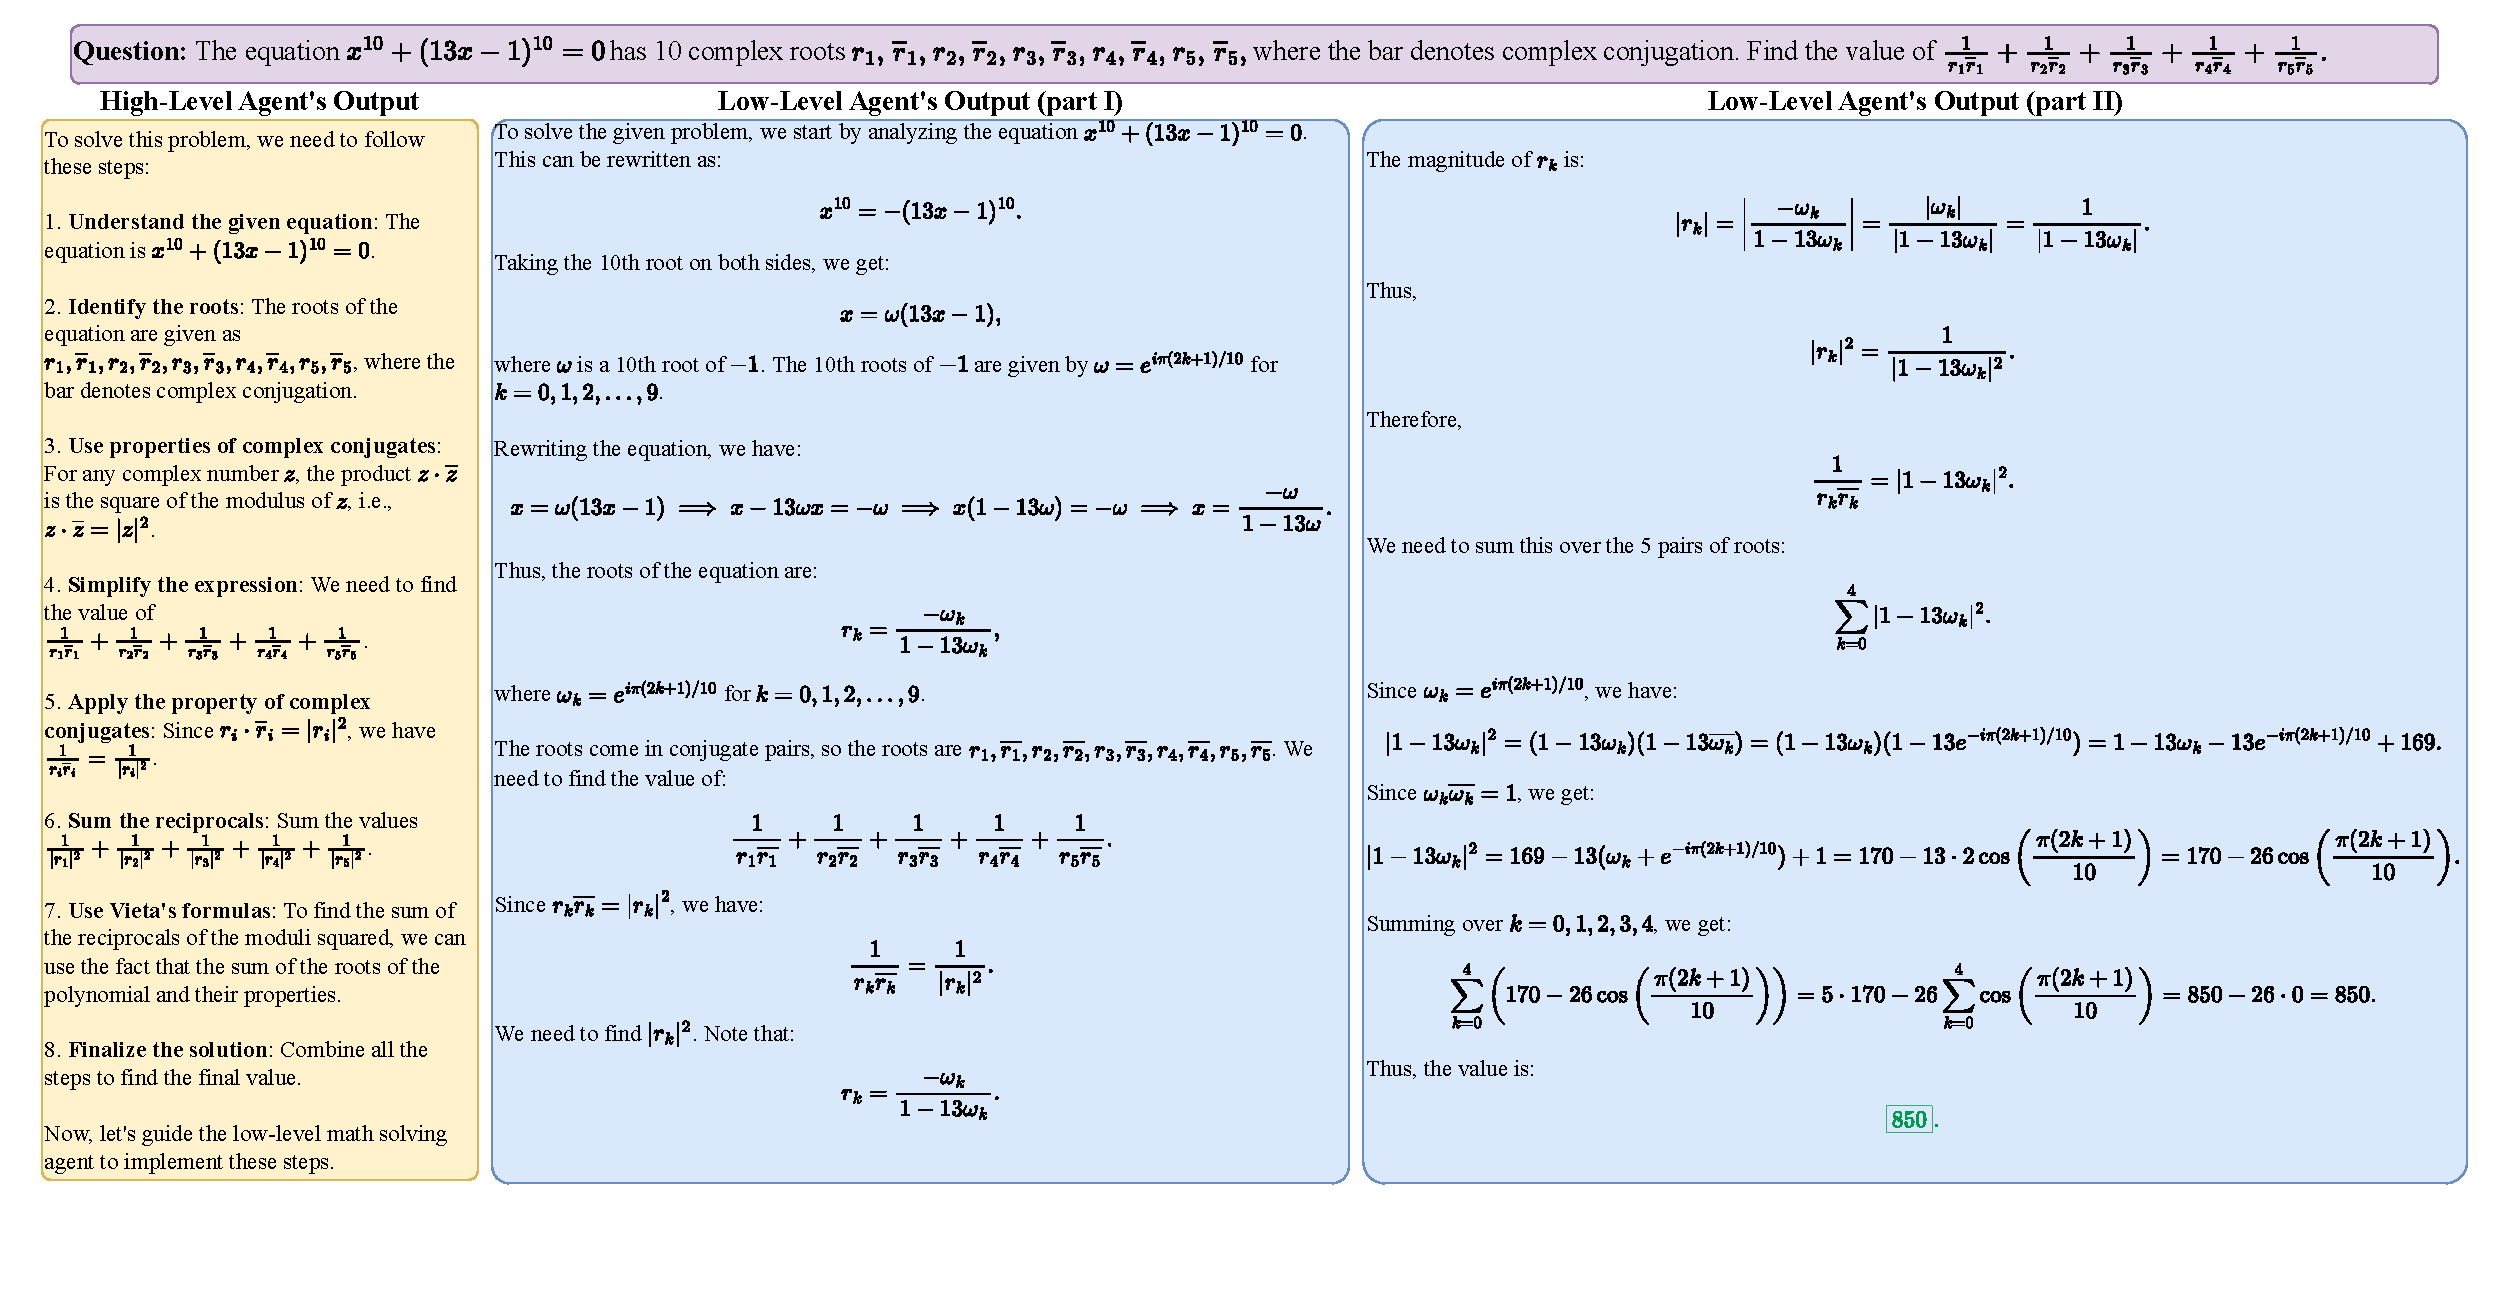
\includegraphics[width=1.0\linewidth]{figures/reward_design_case_studies/exp_reward_design_case_study2.pdf}
    \caption{Case Study for base correctness reward of high-level agent}
    \label{fig:qualative_results.reward_design.case_study2}
\end{figure}

\subsection{Case study for Experiments in Section~\ref{sec:exp.high_rl}}
\label{app:qualative_results.case_study.json}
Fig.~\ref{fig:app.case_study_json} shows the detailed outputs of the two groups of LLMs trained in JSON action.
The outputs finally converge to relative easier and shorter sentences, compared to our main experiments. This may due to insufficient capacity of a small LM to produce a valid JSON-format response while simultaneously exploring diverse reasoning strategies.

\begin{figure}[h!]
    \centering
    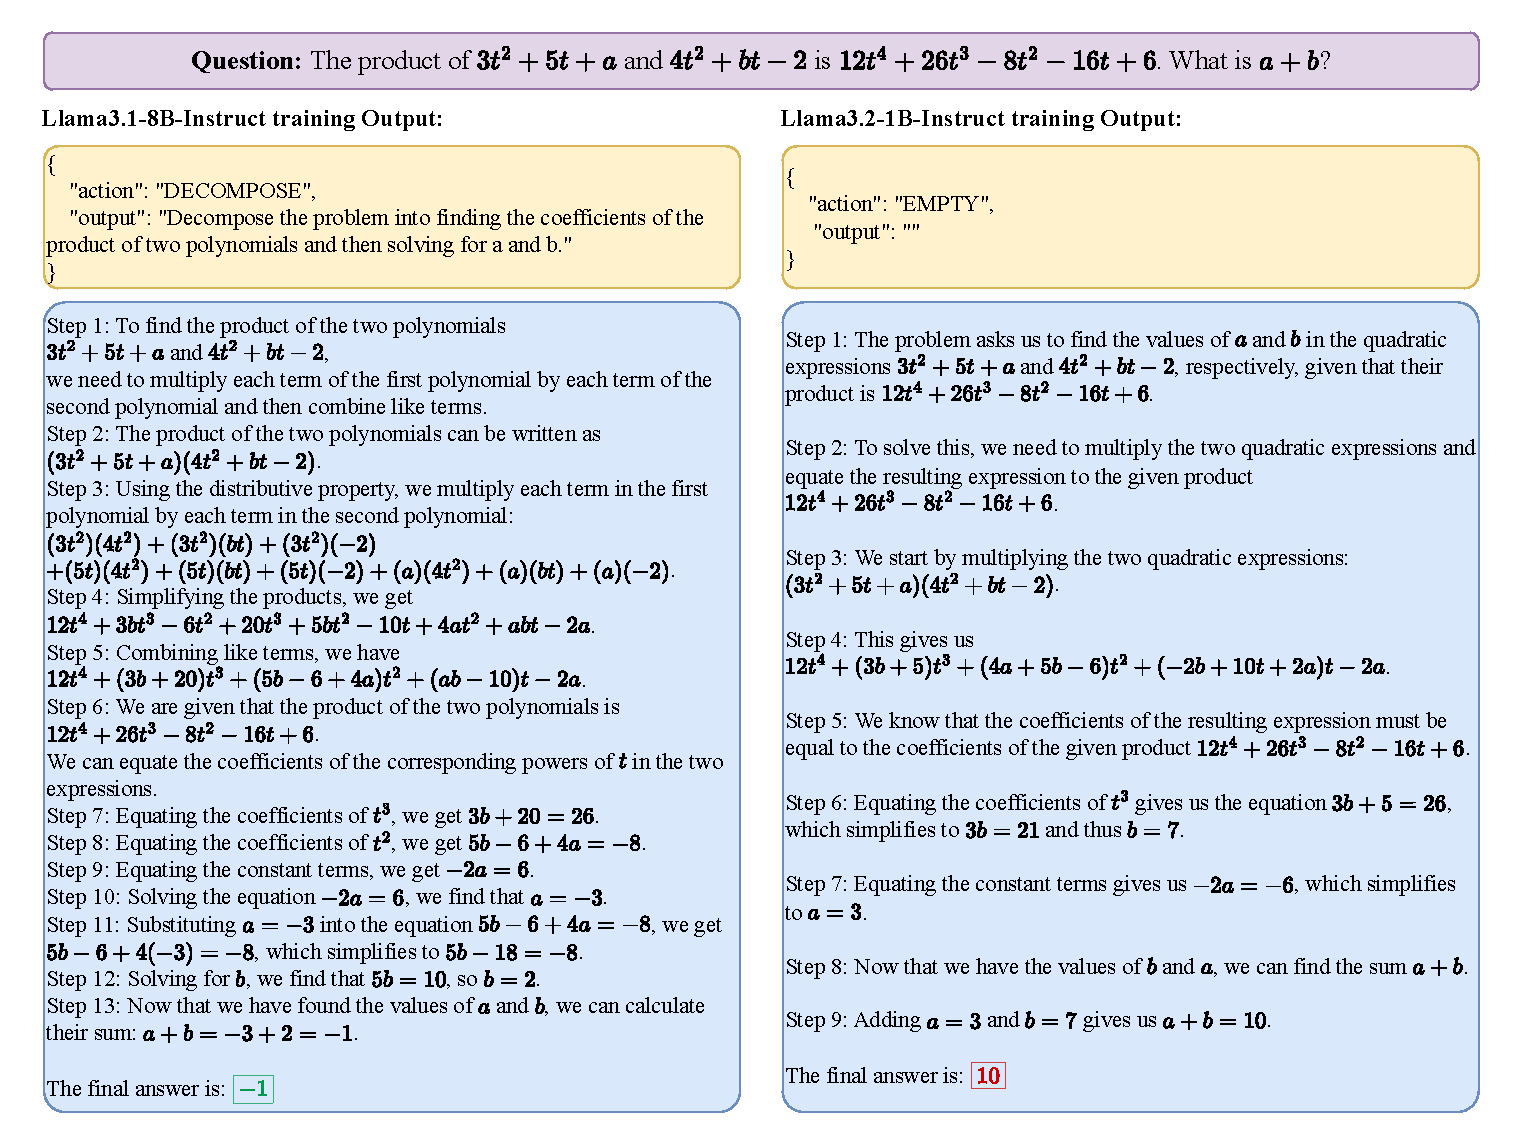
\includegraphics[width=1.0\linewidth]{figures/json_act_case_studies/case_study_json.pdf}
    \caption{Case Study for interpretability experiments in Section~\ref{sec:exp.high_rl}}
    \label{fig:app.case_study_json}
\end{figure}

% \subsection{Qualitative Results of LLM-as-a-Judge}
% Fig~\ref{fig:qualitative_results.laaj.vrp_rl, fig:qualitative_results.laaj.mrp_rl, fig:qualitative_results.laaj.method} show outputs of different methods on LLM-as-a-Judge.

% \begin{figure}[h!]
%     \centering
%     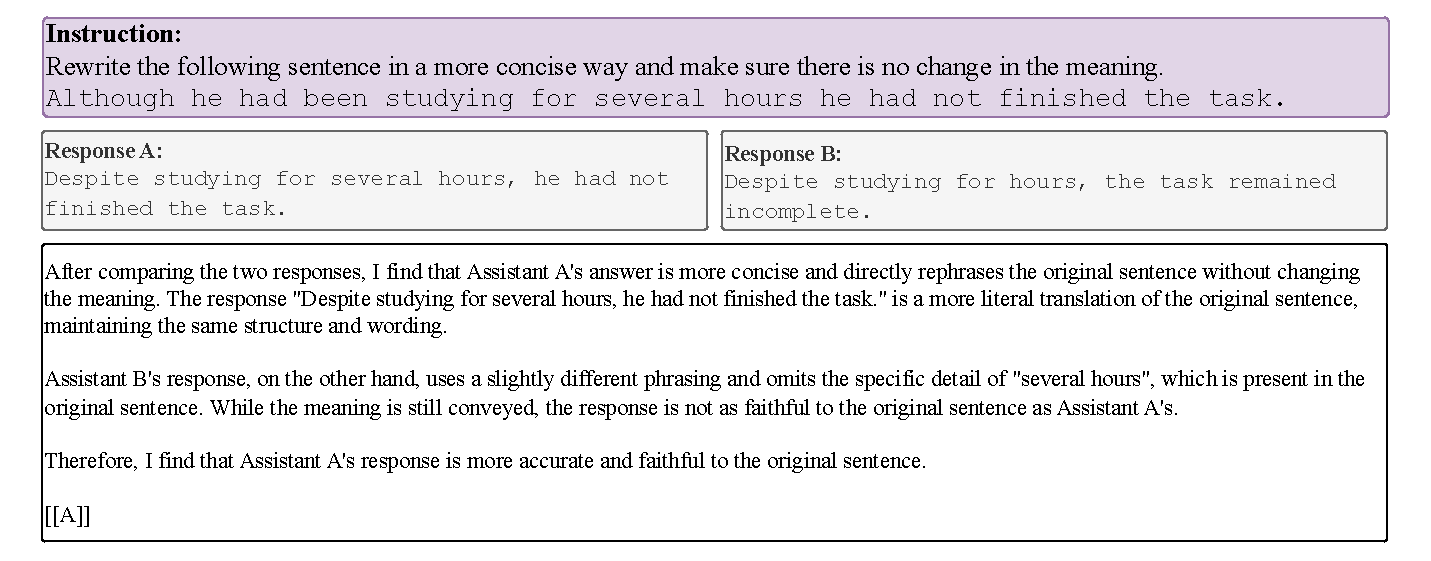
\includegraphics[width=1.0\linewidth]{figures/qualitative_results/laaj_vrp_rl.pdf}
%     \caption{Qualitative Results of VRP$_\text{RL}$ on LLM-as-a-Judge}
%     \label{fig:qualitative_results.laaj.vrp_rl}
% \end{figure}

% \begin{figure}[h!]
%     \centering
%     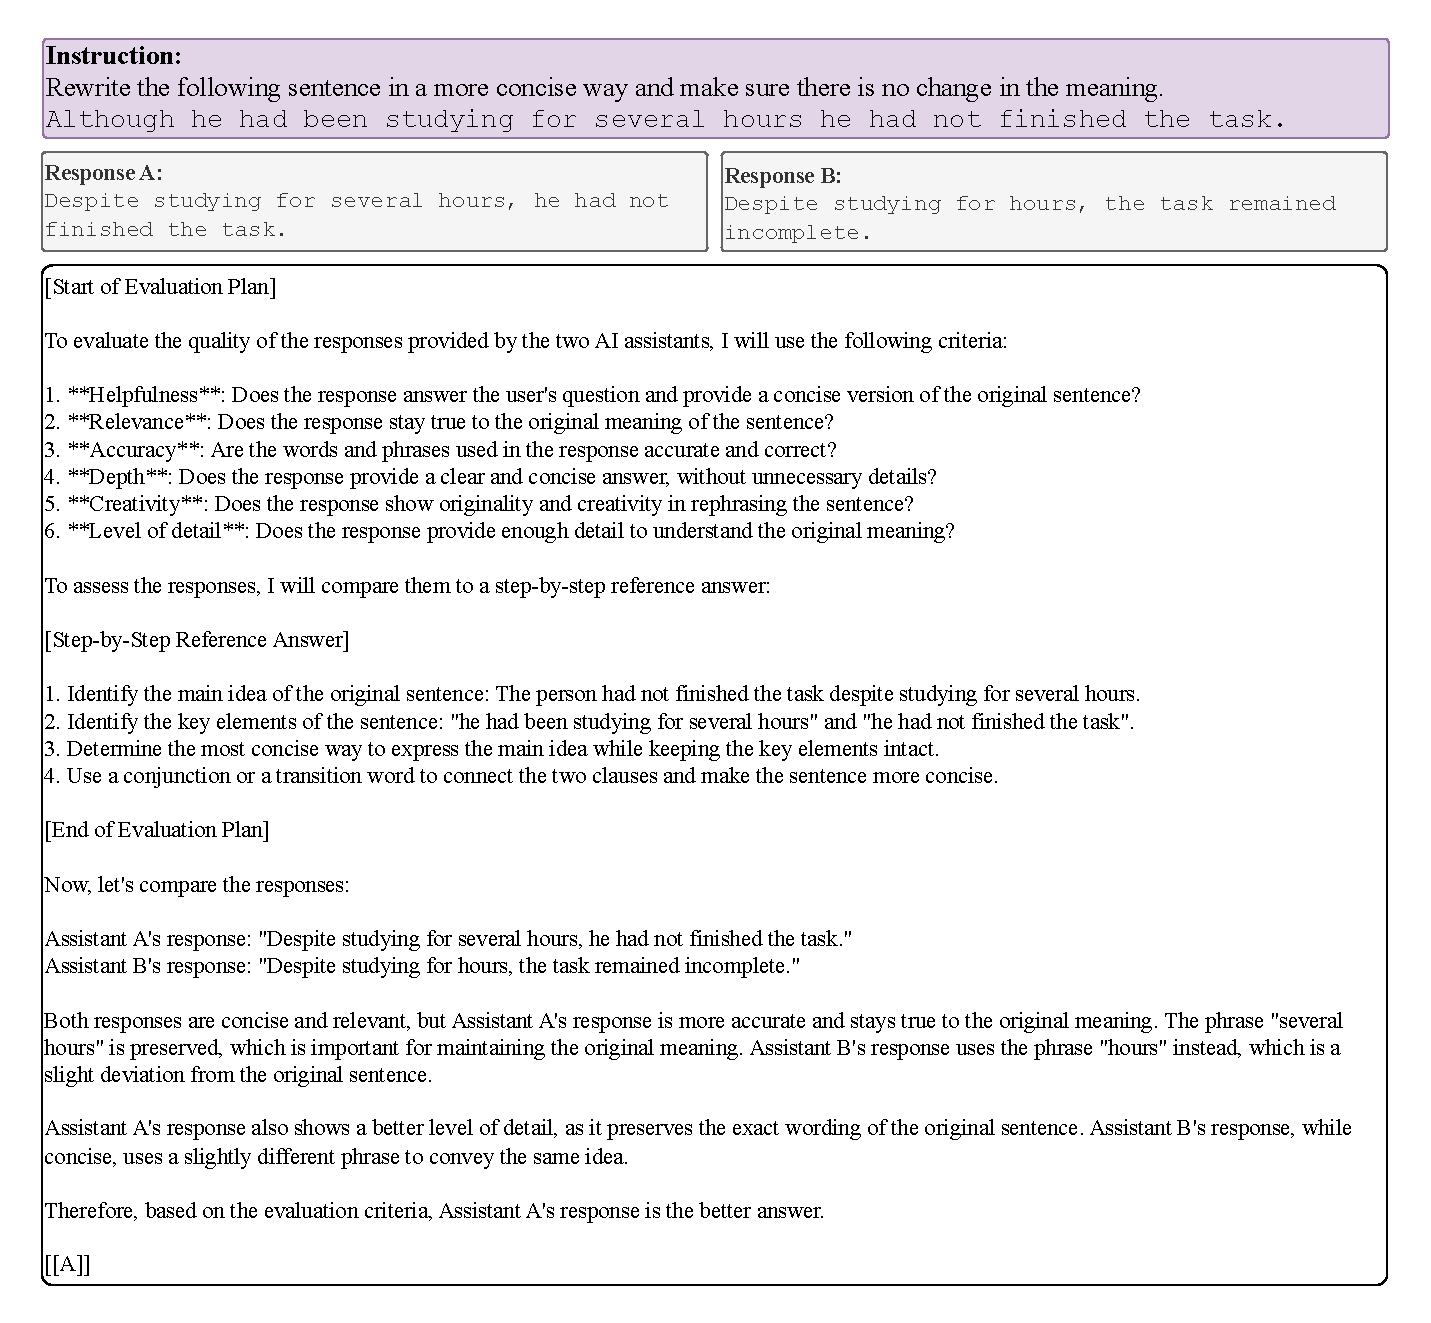
\includegraphics[width=1.0\linewidth]{figures/qualitative_results/laaj_mrp_rl.pdf}
%     \caption{Qualitative Results of MRP$_\text{RL}$ on LLM-as-a-Judge}
%     \label{fig:qualitative_results.laaj.mrp_rl}
% \end{figure}


% \begin{figure}[h!]
%     \centering
%     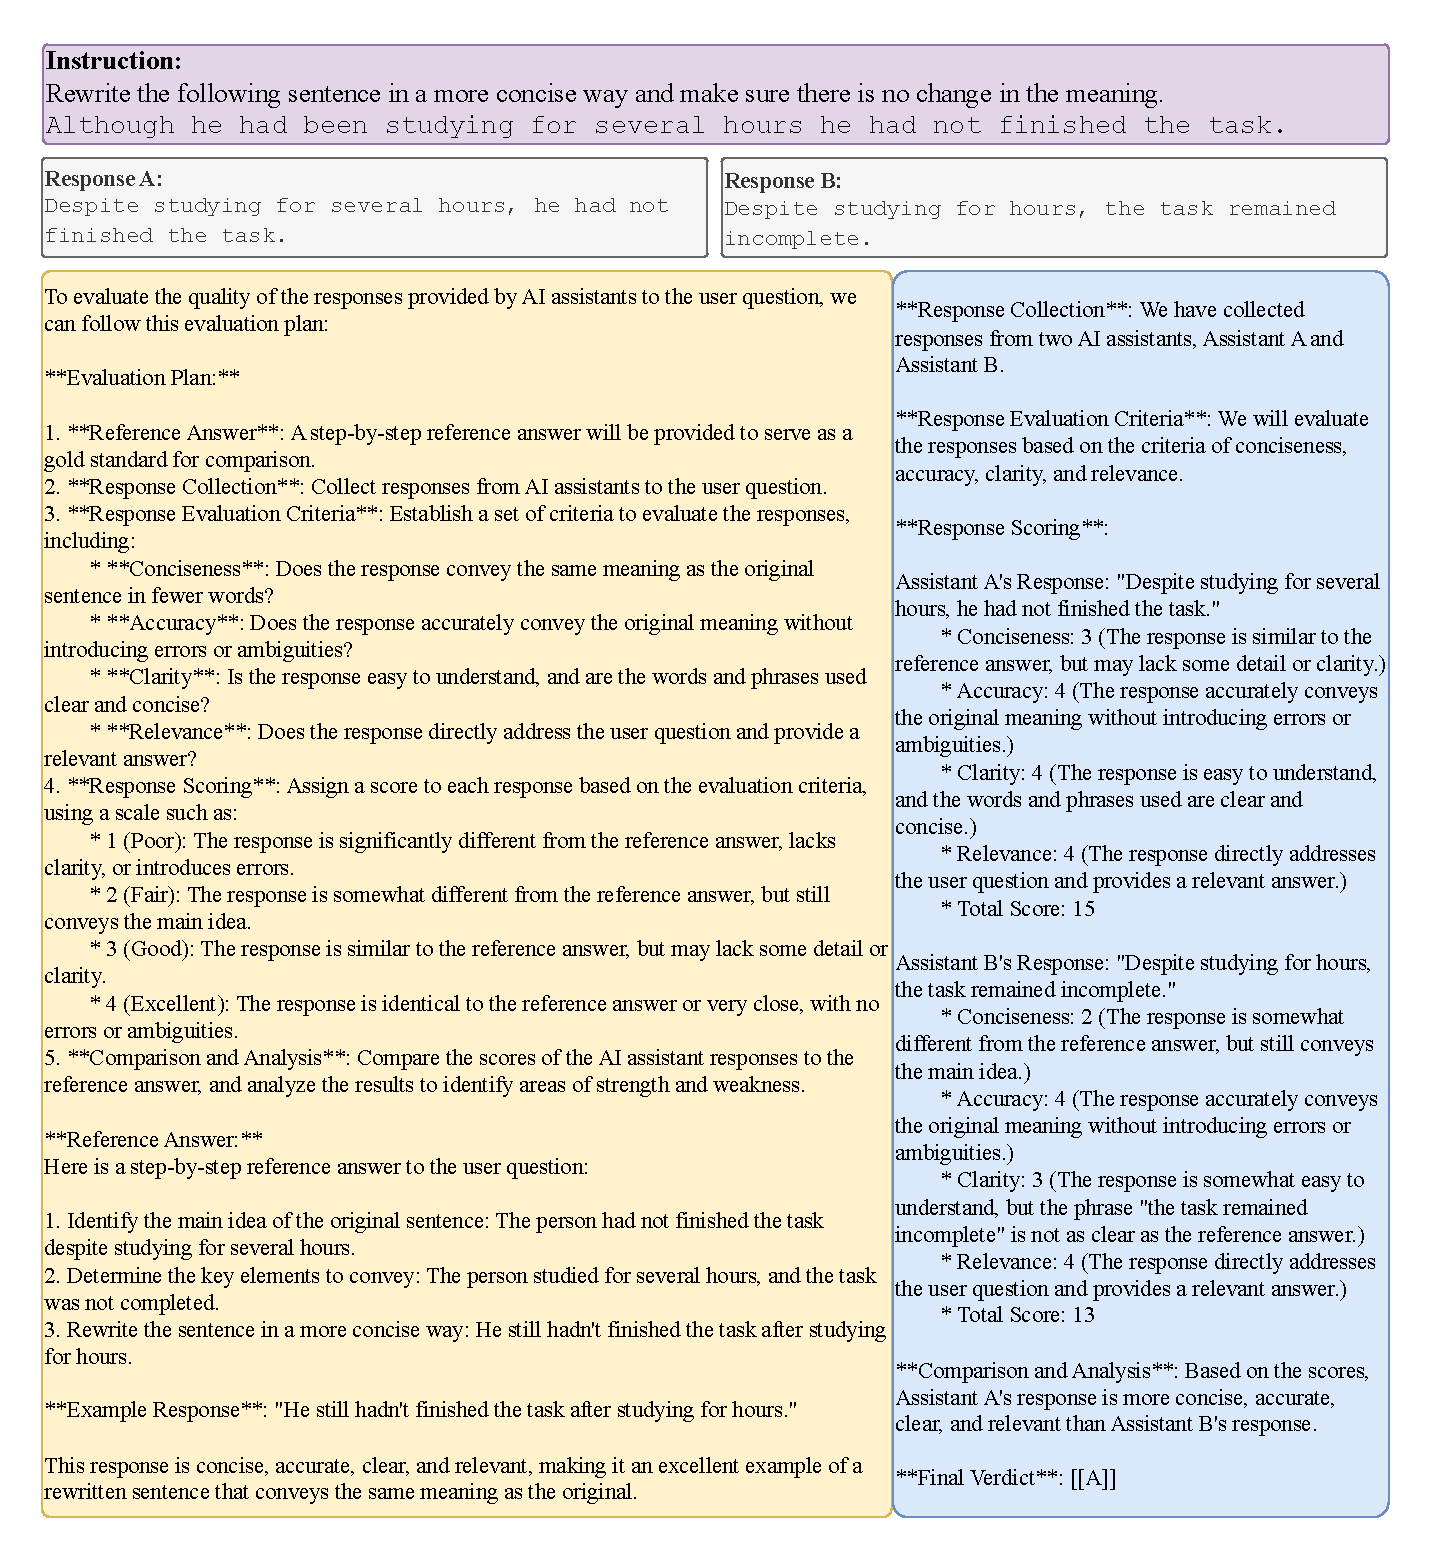
\includegraphics[width=1.0\linewidth]{figures/qualitative_results/llm_as_a_judge.pdf}
%     \caption{Qualitative Results of \method~on LLM-as-a-Judge}
%     \label{fig:qualitative_results.laaj.method}
% \end{figure}

\newpage
\section{Prompts}
\label{app:prompts}
\subsection{Single-turn ReMA prompts}
\label{app:prompts.single_turn_rema}
\subsubsection{Prompts for JSON data collection}
\label{app:prompts.single_turn_rema.json_data}
Prompt for metacognition reasoning to rewrite:
% \begin{lstlisting}[language=XML]
% system_prompt:
%   You are a math expert trying to solve mathematical problems. 
%   Before answering a question, your task is to rewrite the original 
%   question to make it clearer.

%   Provide your rewritten content in JSON format:

%   {{
%   "action": "REWRITE",
%   "output": "{{clearer question content}}"
%   }}

%   Respond only with valid JSON. Do not write an introduction or summary.

% user_prompt:
%   Here is the question:
%   [problem_text]
% \end{lstlisting}

\noindent\fbox{\parbox{\textwidth}{System prompt:

\ttfamily
You are a math expert trying to solve mathematical problems. Before answering a question, your task is to rewrite the original question to make it clearer.

Provide your rewritten content in JSON format:

\{\{

"action": "REWRITE",
"output": "\{\{clearer question content\}\}"

\}\}

Respond only with valid JSON. Do not write an introduction or summary.
\normalfont 

User prompt:

\ttfamily
Here is the question:

[problem\_text]
\normalfont 
}}

Prompt for metacognition reasoning to decompose:

\noindent\fbox{\parbox{\textwidth}{System prompt:

\ttfamily
You are a math expert trying to solve mathematical problems. Before answering a question, your task is to decompose the original question to make it clearer.

Provide your rewritten content in JSON format:

\{\{

"action": "DECOMPOSE",
"output": "\{\{decomposed question content\}\}"

\}\}

Respond only with valid JSON. Do not write an introduction or summary.
\normalfont 

User prompt:

\ttfamily
Here is the question:

[problem\_text]
\normalfont 
}}

Prompt for generating final answers using on the question and metacognition reasoning:

\noindent\fbox{\parbox{\textwidth}{System prompt:

\ttfamily
You are a math expert tasked with solving problems step by step. Follow the provided instructions precisely, showing all reasoning and intermediate steps.

Present the final answer within \textbackslash boxed\{\{\}\}.
\normalfont 

User prompt:

\ttfamily
Here is the question and instructions:

Question

[problem\_text]

Provided Instruction

[instruction\_text]
\normalfont 
}}

\newpage
\subsubsection{Prompts for Math problems}
\label{app:prompts.single_turn_rema.math}
\textbf{VRP prompt:}\\
\noindent\fbox{\parbox{\textwidth}{System prompt:

\ttfamily
You are a math expert tasked with solving problems step by step. 
Present the final answer within \textbackslash boxed\{\}.
\normalfont 

User prompt:

\ttfamily
Here is the question:

\{Question\}
\normalfont 
}}

\textbf{MRP prompt:}\\
\noindent\fbox{\parbox{\textwidth}{System prompt:

\ttfamily
You are a math expert tasked with solving problems. 
When solving a problem, your first task is to provide a high-level solution plan as an instruction.
Then you need to follow the provided instructions precisely, showing all reasoning and intermediate steps.
Finally, you must present the final answer within \textbackslash boxed\{\}.
\normalfont 

User prompt:

\ttfamily
Here is the question:

\{Question\}
\normalfont 
}}

\textbf{MAMRP prompt:}\\
high-level agent:\\
\noindent\fbox{\parbox{\textwidth}{System prompt:

\ttfamily
You are a math expert specialized in solving mathematical problems, you need to teach a weaker agent with minimal capability in math how to solve a problem step-by-step. 

Your task is to provide a high-level solution plan for the given problem, in order to guide a low-level math solving agent to solve the problem.

You can not directly answer the question. You'll be punished if you include any answer in your response.

You need to first think deeply in mind and output your final instruction.
\normalfont 

User prompt:

\ttfamily
Here is the question:

\{Question\}
\normalfont 
}}
low-level agent:\\
\noindent\fbox{\parbox{\textwidth}{System prompt:

\ttfamily
You are a math expert tasked with solving problems step by step. Follow the provided instructions precisely, showing all reasoning and intermediate steps.
Present the final answer within \textbackslash boxed\{\}.

\normalfont 

User prompt:

\ttfamily
Here is the question and instructions:\\

[Question]

\{Question\}

[End of Question]\\

[Provided Instruction]

\{instruction\}

[End of Instruction]
\normalfont 
}}

\newpage
\subsubsection{Prompts for LLM-as-a-Judge problems}
\label{app:prompts.single_turn_rema.llm_as_a_judge}
We adopt the prompts from \citet{saha2025learning}. \\
\textbf{VRP prompt:}\\
\noindent\fbox{\parbox{\textwidth}{System prompt:

\ttfamily
Please act as an impartial judge and evaluate the quality of the responses provided by two AI assistants to the user question displayed below. You should choose the assistant that follows the user's instructions and answers the user's question better. 

Your evaluation should consider factors such as the helpfulness, relevance, accuracy, depth, creativity, and level of detail of their responses. Begin your evaluation by comparing the two responses and provide a short explanation. Avoid any position biases and ensure that the order in which the responses were presented does not influence your decision. 

Do not allow the length of the responses to influence your evaluation. 

Do not favor certain names of the assistants. Be as objective as possible. After providing your explanation, output your final verdict by strictly following this format: "[[A]]" if assistant A is better, "[[B]]" if assistant B is better.
\normalfont 

User prompt:

\ttfamily
[User Question]

\{instruction\}

[End of User Question]

[The Start of Assistant A's Answer]

\{response\_A\}

[The End of Assistant A's Answer]

[The Start of Assistant B's Answer]

\{response\_B\}

[The End of Assistant B's Answer]

\normalfont 
}}

\newpage
\textbf{MRP prompt:}\\
\noindent\fbox{\parbox{\textwidth}{System prompt:

\ttfamily
Please act as an impartial judge and evaluate the quality of the responses provided by two AI assistants to the user question displayed below. You should choose the assistant that follows the user's instructions and answers the user's question better. 

First of your task is to build an evaluation plan that can then be executed to assess the response quality. Whenever appropriate, you can choose to also include a step-by-step reference answer as part of the evaluation plan. 

Enclose your evaluation plan between the tags "[Start of Evaluation Plan]" and "[End of Evaluation Plan]".

After that, please act as an impartial judge and evaluate the quality of the responses provided by two AI assistants to the user question displayed below. You should choose the assistant that follows the user's instructions and answers the user's question better. 

Your evaluation should consider factors such as the helpfulness, relevance, accuracy, depth, creativity, and level of detail of their responses. Begin your evaluation by comparing the two responses and provide a short explanation. Avoid any position biases and ensure that the order in which the responses were presented does not influence your decision. 

Do not allow the length of the responses to influence your evaluation. 

Do not favor certain names of the assistants. Be as objective as possible. After providing your explanation, output your final verdict by strictly following this format: "[[A]]" if assistant A is better, "[[B]]" if assistant B is better.

\normalfont 

User prompt:

\ttfamily
[User Question]

\{instruction\}

[End of User Question]

[The Start of Assistant A's Answer]

\{response\_A\}

[The End of Assistant A's Answer]

[The Start of Assistant B's Answer]

\{response\_B\}

[The End of Assistant B's Answer]
\normalfont 
}}

\textbf{MAMRP prompt:}
high-level agent:\\
\noindent\fbox{\parbox{\textwidth}{System prompt:

\ttfamily
We want to evaluate the quality of the responses provided by AI assistants to the user question displayed below. 

For that, your task is to help us build an evaluation plan that can then be executed to assess the response quality. Whenever appropriate, you can choose to also include a step-by-step reference answer as part of the evaluation plan. 
\normalfont 

User prompt:

\ttfamily
[User Question]

\{Question\}

[End of User Question]
\normalfont 
}}

low-level agent:\\
\noindent\fbox{\parbox{\textwidth}{System prompt:

\ttfamily
Please act as an impartial judge and evaluate the quality of the responses provided by two AI assistants to the user question displayed below. Your evaluation should be performed by following the provided evaluation plan step-by-step. Avoid copying the plan when doing the evaluation. 

Please also only stick to the given plan and provide explanation of how the plan is executed to compare the two responses. 

Avoid any position biases and ensure that the order in which the responses were presented does not influence your decision. 

Do not allow the length of the responses to influence your evaluation. Do not favor certain names of the assistants. Be as objective as possible. 

After providing your evaluation, output your final verdict by strictly following this format: "[[A]]" if assistant A is better, "[[B]]" if assistant B is better.

\normalfont 

User prompt:

\ttfamily

[User Question]

\{instruction\}

[End of User Question]

[The Start of Assistant A's Answer]

\{response\_A\}

[The End of Assistant A's Answer]

[The Start of Assistant B's Answer]

\{response\_B\}

[The End of Assistant B's Answer]

[The Start of Evaluation Plan]

\{evaluation\_plan\}

[The End of Evaluation Plan]

\normalfont 
}}

\subsection{Multi-turn ReMA prompts}
\label{app:prompts.multi_turn_rema}
\subsubsection{SFT data collection of multi-turn MAMRP}
\label{app:prompts.multi_turn_rema.sft_data}

\noindent\fbox{\parbox{\textwidth}{System prompt:

\ttfamily
You are classifying reasoning process data into two types of thinking. You will be given a question-answer pair from a reasoning dataset. Your task is to split all words into two parts. These words are crucial for analyzing reasoning patterns, so do not skip any details.


- **Meta-Thinking Agent (MTA):** Responsible for high-level thought processes. This includes planning, evaluating steps, expressing uncertainty, making observations, or setting goals. Avoid detailed calculations. The content should be enclosed in `<meta\_thinking>` and `</meta\_thinking>`.  

- **Reasoning Agent (RA):** Responsible for detailed problem-solving steps, such as calculations, logical deductions, or breaking down a problem into subproblems. The content should be enclosed in `<reasoning>` and `</reasoning>`.  

**Rules to follow:**

1. **Do not assign large chunks of text to a single type of thinking.** The reasoning process consists of small, nonlinear thinking steps, so alternate appropriately between Meta-Thinking and Reasoning steps.  

2. **Keep the words from the original solution unmodified whenever possible.** Words like "Wait," "Hmm," "But," etc., typically indicate Meta-Thinking and should be preserved. 

3. **When finalizing the answer:**

\indent- The **Meta-Thinking Agent (MTA)** must explicitly confirm the answer before completion and output `[FINISH]`.  
   
\indent- The **Reasoning Agent (RA)** should then provide the final answer in the correct format.  

4. **Do not skip any reasoning steps, even if they seem redundant, incorrect or irrelevant**  

5. **Do not modify or remove any part of the original reasoning process**, even if it seems redundant or repetitive. The goal is to **preserve the exact flow of thought** as it naturally occurs.

6. **Retain all expressions such as "Wait," "Hmm," "But wait," etc., exactly as they appear. These indicate important cognitive processes and should not be skipped or altered.**


Here are examples for you:

[Examples]
...

\normalfont 

User prompt:

\ttfamily

[Begin of Question]

\{question\}

[End of Question]

[Begin of Solution]

\{solution\}

[End of Solution]

\normalfont 
}}

\newpage
\subsubsection{Prompt for math problems}
\label{app:prompts.multi_turn_rema.math}

\textbf{Meta-Thinking Agent (MTA):}

\noindent\fbox{\parbox{\textwidth}{System prompt:

\ttfamily
You are a meta-think agent that represents human high-level think process, when solving a question, you will have a discussion with human, each time you think about what to do next: e.g. 

- Exploring multiple angles and approaches

- Breaking down the solution into clear steps

- Continuously reflecting on intermediate results honestly and adapt your strategy as you progress

- Backtracking when necessary

- Requesting exploration of multiple solutions individually

- Finally confirm the answer with the tag [FINISH]

User prompt:

\ttfamily

\{question\}

\normalfont 
}}

\textbf{Reasoning Agent (RA):}

\noindent\fbox{\parbox{\textwidth}{System prompt:

\ttfamily
Please reason step by step follow the given instruction, when asked to finalize your answer, put your answer within \textbackslash boxed\{\}

\normalfont
User prompt:

\ttfamily

\{question\}

\{instruction\}

\normalfont 
}}